\documentclass[11pt,a4paper,oneside]{report}

% ---------------------------------------------------------
% Core Packages and Typography
% ---------------------------------------------------------
\usepackage[utf8]{inputenc}
\usepackage[T1]{fontenc}
\usepackage{lmodern}
\usepackage{amsmath,amssymb,amsfonts,amsthm,mathtools}
\usepackage[margin=1in,headheight=14pt]{geometry}
\usepackage{graphicx}
\usepackage{booktabs}
\usepackage{tabularx}
\usepackage{multirow}
\usepackage{multicol}
\usepackage{array}
\usepackage{xcolor}
\usepackage{fancyhdr}
\usepackage{titlesec}
\usepackage{caption}
\usepackage{subcaption}
\usepackage{listings}
\usepackage{algorithm}
\usepackage{algpseudocode}
\usepackage{microtype}
\usepackage{setspace}
\usepackage{tikz}
\usetikzlibrary{shapes,arrows,positioning,calc}

% Define color palette
\definecolor{vjtiMaroon}{RGB}{128, 0, 0}
\definecolor{navyBlue}{RGB}{0, 32, 96}
\definecolor{darkSlate}{RGB}{47, 79, 79}
\definecolor{lightGray}{RGB}{245, 245, 245}
\definecolor{codegreen}{rgb}{0,0.6,0}
\definecolor{codegray}{rgb}{0.5,0.5,0.5}
\definecolor{codepurple}{rgb}{0.58,0,0.82}

\usepackage[
    colorlinks=true,
    linkcolor=navyBlue,
    citecolor=vjtiMaroon,
    urlcolor=darkSlate,
    bookmarks=true,
    bookmarksnumbered=true
]{hyperref}

% Page styling
\pagestyle{fancy}
\fancyhf{}
\fancyhead[L]{\small\nouppercase{\leftmark}}
\fancyhead[R]{\small\thepage}
\renewcommand{\headrulewidth}{0.5pt}
\renewcommand{\footrulewidth}{0pt}

% Section title formatting
\titleformat{\chapter}[display]
  {\normalfont\huge\bfseries\color{vjtiMaroon}}{\chaptertitlename\ \thechapter}{20pt}{\Huge}
\titlespacing*{\chapter}{0pt}{10pt}{25pt}

\onehalfspacing

% Code listing configuration
\lstset{
    backgroundcolor=\color{lightGray},
    basicstyle=\ttfamily\footnotesize,
    breakatwhitespace=false,
    breaklines=true,
    captionpos=b,
    commentstyle=\color{codegreen},
    keywordstyle=\color{navyBlue}\bfseries,
    numberstyle=\tiny\color{codegray},
    numbers=left,
    numbersep=5pt,
    showspaces=false,
    showstringspaces=false,
    showtabs=false,
    stringstyle=\color{codepurple},
    tabsize=2
}

\begin{document}

% ---------------------------------------------------------
% Title Page
% ---------------------------------------------------------
\begin{titlepage}
    \centering
    \vspace*{0.5cm}
    
    {\Huge \bfseries \color{vjtiMaroon} VEERMATA JIJABAI TECHNOLOGICAL INSTITUTE}\\[0.3cm]
    {\Large \bfseries (VJTI Mumbai)}\\[0.2cm]
    {\normalsize Central Technical Institute, Matunga, Mumbai, Maharashtra 400019}\\[1.2cm]
    
    \hrule height 1.5pt \vspace{0.4cm}
    {\huge \bfseries Fair and Load-Balanced Multi-Objective Student-Alumni Matching}\\[0.4cm]
    {\LARGE \bfseries Capacitated Bipartite Assignment with Rawlsian Egalitarianism and Departmental Parity}\\[0.4cm]
    \hrule height 1.5pt \vspace{1.2cm}
    
    \begin{minipage}{0.48\textwidth}
        \flushleft
        \textbf{\large Course:} Optimization Techniques (OT)\\
        \textbf{\large Program:} B.Tech / M.Tech Elective\\
        \textbf{\large Academic Year:} 2026--2027
    \end{minipage}
    \hfill
    \begin{minipage}{0.48\textwidth}
        \flushright
        \textbf{\large Project Category:} Mini-Project Implementation\\
        \textbf{\large Target Audience:} Academic Review Board\\
        \textbf{\large Department:} Computer Engineering \& IT
    \end{minipage}
    
    \vfill
    
    \begin{minipage}{0.9\textwidth}
        \centering
        \small
        \textbf{Statutory Compliance and Privacy Notice:}\\
        \textit{All student profiles, alumni profiles, departmental affinities, corporate associations, and compatibility matrices utilized throughout this report are strictly artificial and synthesized for scientific testing only. Pseudonymous identifiers (\texttt{S001}--\texttt{S1000}, \texttt{A001}--\texttt{A500}) are employed throughout. No real Personally Identifiable Information (PII) or institutional database records were queried or stored.}
    \end{minipage}
    
    \vspace{1cm}
    {\large \today}
\end{titlepage}

% ---------------------------------------------------------
% Front Matter
% ---------------------------------------------------------
\pagenumbering{roman}
\tableofcontents
\newpage
\listoffigures
\newpage
\listoftables
\newpage

% ---------------------------------------------------------
% Executive Summary
% ---------------------------------------------------------
\chapter*{Executive Summary}
\addcontentsline{toc}{chapter}{Executive Summary}

Alumni mentorship programs within premier technological universities serve as foundational pillars bridging academic foundational coursework with contemporary industrial practice. At \textbf{Veermata Jijabai Technological Institute (VJTI), Mumbai}, matching students across eight specialized engineering departments with an expansive alumni network presents high-dimensional combinatorial challenges. Historically, institutional allocations have relied upon ad-hoc heuristic sorting or greedy score-first priority assignments. 

In this comprehensive report, we model the institutional assignment challenge as a formal \textbf{Multi-Objective Capacitated Bipartite Assignment Problem (MO-CBAP)}. We formalize three fundamentally competing objectives:
\begin{enumerate}
    \item \textbf{Utilitarian Placement Efficiency ($Z_1$)}: Maximizing the aggregate pairwise compatibility across all student-alumni assignments.
    \item \textbf{Rawlsian Egalitarian Fairness ($Z_2$)}: Maximizing the match quality of the most vulnerable, least-advantaged student ($\min_i Q_i$), safeguarding against peripheral neglect.
    \item \textbf{Alumni Workload Balancing ($Z_3$)}: Minimizing the maximum mentorship burden assigned to any single alumnus ($\max_j L_j$), actively mitigating burnout in high-demand industry profiles.
\end{enumerate}

To enforce institutional policies, we impose seven operational constraints including individual capacities, opt-in consent compliance, student quality floors ($\theta$), cross-departmental branch parity caps ($\delta$), corporate diversity caps, and exact degree requirements.

We evaluate an extensive algorithmic portfolio spanning:
\begin{itemize}
    \item \textbf{Deterministic and Stochastic Baselines}: Random Feasible, Greedy Score-First, and Single-Objective Min-Cost Flow (with both raw and repaired diversity variants).
    \item \textbf{Exact Mathematical Solvers}: Mixed-Integer Linear Programming (MILP) solved via HiGHS using Weighted-Sum and $\epsilon$-Constraint sweeps to establish true Pareto optimality benchmarks on small cohorts.
    \item \textbf{Evolutionary Multi-Objective Optimizers}: Standard NSGA-II, SPEA2, and MOEA/D under uniform evaluation budgets.
    \item \textbf{Hybrid Memetic NSGA-II}: A specialized algorithm combining heuristic seed initialization (Greedy, Rawlsian-priority, and Workload-balanced) with Lamarckian 2-opt swaps and Pareto elitist archiving.
\end{itemize}

Empirical evaluations executed across 30 independent seeds under a unified, normalized shared Hypervolume reference frame establish that the \textbf{Hybrid Memetic NSGA-II} delivers statistically superior results ($p = 1.86 \times 10^{-9}$, effect size $r = 1.00$). On the $50 \times 30$ cohort, the Hybrid achieves a mean Hypervolume of \textbf{0.7650} (compared to \textbf{0.3648} for NSGA-II, \textbf{0.3739} for SPEA2, and \textbf{0.0932} for Greedy), simultaneously elevating worst-student satisfaction from 0.5468 to 1.1276 and suppressing peak alumni load from 8 to 5.53. Crucially, the Hybrid Pareto front dominates the single-point Greedy baseline in 100\% of trial runs. We conclude with comprehensive ablation analyses, threshold calibrations, sensitivity assessments, and concrete institutional deployment guidelines.

\newpage
\pagenumbering{arabic}

% ---------------------------------------------------------
% Main Chapters
% ---------------------------------------------------------
\chapter{Introduction and Problem Motivation}
\label{ch:intro}

\section{Institutional Context: VJTI Alumni Mentorship Ecosystem}
Established in 1887, Veermata Jijabai Technological Institute (VJTI) in Matunga, Mumbai, stands as one of India's preeminent engineering colleges. Across eight specialized undergraduate and postgraduate academic departments—Computer Engineering (\texttt{CE}), Information Technology (\texttt{IT}), Electronics and Telecommunication Engineering (\texttt{EXTC}), Electrical Engineering (\texttt{EE}), Mechanical Engineering (\texttt{ME}), Civil and Environmental Engineering (\texttt{CEV}), Production Engineering (\texttt{PE}), and Textile Technology (\texttt{TT})—graduating cohorts seek industry exposure.

Alumni mentorship programs provide undergraduate engineers with direct vocational advisory, technical portfolio reviews, career roadmap structuring, and professional networking. Modern career aspirations are inherently multidimensional, encompassing six broad industrial sectors:
\begin{enumerate}
    \item \textbf{Software \& Artificial Intelligence}: Core algorithm design, cloud computing, enterprise software architectures, and machine learning infrastructure.
    \item \textbf{Data Science \& Advanced Analytics}: Quantitative modeling, statistical inference, data engineering pipelines, and business intelligence.
    \item \textbf{Electronics \& Embedded Systems}: VLSI design, semiconductor manufacturing, IoT hardware engineering, and robotics control firmware.
    \item \textbf{Core Engineering \& Manufacturing}: Automotive dynamics, heavy machinery, thermodynamics, structural engineering, and smart manufacturing.
    \item \textbf{Finance \& Quantitative Trading}: Algorithmic execution, financial econometrics, risk modeling, and FinTech systems.
    \item \textbf{Management Consulting \& Corporate Strategy}: Operational optimization, technical management consulting, supply chain analytics, and market assessment.
\end{enumerate}

\section{Operational Pathologies in Conventional Mentorship Systems}
Despite the high stakes of mentor allocations, prevailing administrative paradigms in tertiary institutions frequently rely upon unconstrained self-selection, spreadsheet-driven manual pairing, or first-come-first-served greedy allocation algorithms. In practice, these legacy approaches suffer from three acute structural pathologies:

\begin{figure}[htbp]
    \centering
    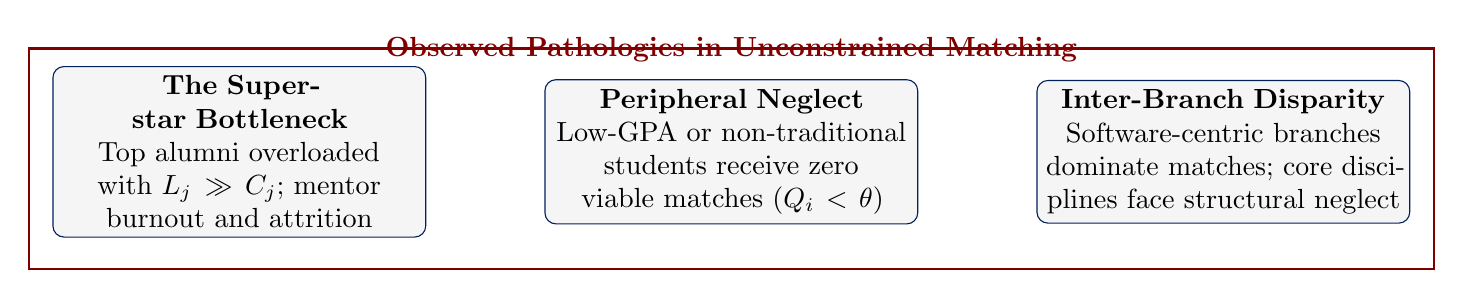
\begin{tikzpicture}[node distance=1.5cm, auto,
        block/.style={rectangle, draw=navyBlue, fill=lightGray, text width=4.5cm, text centered, rounded corners, minimum height=1.2cm},
        arrow/.style={thick, ->, >=stealth}]
        
        \node [block] (superstar) {\textbf{The Superstar Bottleneck}\\Top alumni overloaded with $L_j \gg C_j$; mentor burnout and attrition};
        \node [block, right=1.5cm of superstar] (peripheral) {\textbf{Peripheral Neglect}\\Low-GPA or non-traditional students receive zero viable matches ($Q_i < \theta$)};
        \node [block, right=1.5cm of peripheral] (parity) {\textbf{Inter-Branch Disparity}\\Software-centric branches dominate matches; core disciplines face structural neglect};
        
        \draw [thick, color=vjtiMaroon] ($(superstar.south west)+(-0.3,-0.4)$) rectangle ($(parity.north east)+(0.3,0.4)$);
        \node [above=0.1cm of peripheral] {\textbf{\color{vjtiMaroon}Observed Pathologies in Unconstrained Matching}};
    \end{tikzpicture}
    \caption{Structural failure modes induced by unconstrained or purely utilitarian matching mechanisms.}
    \label{fig:pathologies}
\end{figure}

\subsection{The ``Superstar Alumnus'' Bottleneck}
Prominent alumni occupying leadership positions (e.g., Vice Presidents at global technology firms, partners in consulting partnerships, or prominent venture-backed founders) naturally exhibit broad appeal. When matching algorithms prioritize purely unconstrained preference maximization or utilitarian score sums, these ``superstar'' alumni are assigned disproportionately high volumes of students ($L_j \ge 8$). This over-allocation directly triggers cognitive fatigue, delayed feedback loops, superficial mentorship interactions, and eventual mentor attrition from future institutional programs.

\subsection{Peripheral Student Neglect}
Purely utilitarian objectives seek solely to maximize the cumulative sum of pairwise compatibility scores $\sum_{i,j} q_{ij} x_{ij}$. Under this paradigm, high-GPA students possessing stellar academic resumes receive multiple elite mentors. Conversely, students exhibiting average academic metrics, those exploring cross-departmental career shifts, or students from under-represented backgrounds are systematically relegated to residual, poorly aligned matches. In severe cases, realized match quality drops below viable thresholds ($Q_i < \theta$), leaving vulnerable students disenfranchised.

\subsection{Inter-Departmental Parity Gaps}
Because computing disciplines (\texttt{CE}, \texttt{IT}) boast significantly larger and more concentrated alumni cohorts across modern software and financial sectors, an unconstrained algorithm naturally funnels premium resources toward these groups. Conversely, students from vital traditional engineering disciplines (\texttt{PE}, \texttt{CEV}, \texttt{TT}, \texttt{ME}) experience diminished average mentorship quality. Without explicit branch-parity bounds, institutional inequity widens.

\subsection{Corporate Homogeneity}
Students assigned multiple mentors (e.g., $K=2$) risk receiving duplicate assignments from the same corporate employer (e.g., two mentors from the identical enterprise cloud corporation). This diminishes the breadth of student perspective and restricts exposure to contrasting organizational cultures, hiring practices, and career paths.

\section{Research Objectives and Scope}
To overcome these limitations, this research project formulates and solves the \textbf{Multi-Objective Capacitated Bipartite Assignment Problem (MO-CBAP)}. The primary objectives of this investigation are:
\begin{enumerate}
    \item \textbf{Mathematical Formalization}: Rigorously model student-alumni matching as a tri-objective constrained combinatorial optimization problem balancing Utilitarian Efficiency ($Z_1$), Rawlsian Fairness ($Z_2$), and Alumni Workload Balance ($Z_3$) under seven operational constraints.
    \item \textbf{Algorithmic Portfolio Benchmark}: Develop and comparatively evaluate a diverse algorithmic suite including deterministic baselines (Random, Greedy, Min-Cost Flow), exact branch-and-cut MILP solvers, and modern multi-objective evolutionary algorithms (NSGA-II, SPEA2, MOEA/D).
    \item \textbf{Hybrid Memetic Innovation}: Design a specialized domain-aware Memetic NSGA-II incorporating heuristic seeding, Rawlsian-targeted 2-opt local search swaps, workload relief moves, and elitist archiving.
    \item \textbf{Multi-Seed Rigorous Statistics}: Execute 30 independent stochastic runs under unified, normalized shared Hypervolume references, applying non-parametric Wilcoxon signed-rank hypothesis tests with effect sizes ($r$).
    \item \textbf{Parameter Calibration and Sensitivity Analysis}: Provide an empirical calibration framework for institutional parameters ($\theta$, $\delta$) derived from baseline data distributions.
\end{enumerate}

\section{Ethical Considerations and Synthetic Data Governance}
In strict adherence to institutional data governance standards and ethical computational guidelines, \textbf{no personal identifiable information (PII) or real student academic records} were accessed or utilized. All experimental cohorts were synthesized using a reproducible parametric data generator incorporating realistic departmental distributions, domain affinity matrices, and log-normal capacity profiles. Synthetic profiles utilize pseudonymous identifiers (\texttt{S001}--\texttt{S1000}, \texttt{A001}--\texttt{A500}). The resulting optimization framework is inherently privacy-preserving and domain-agnostic.


\chapter{Mathematical Formulation of the MO-CBAP}
\label{ch:formulation}

\section{System Notations and Parameter Definitions}
Let the institutional matching environment be characterized by the following sets and parameters:
\begin{itemize}
    \item $\mathcal{S} = \{1, 2, \dots, N\}$: The finite set of graduating student candidates.
    \item $\mathcal{A} = \{1, 2, \dots, M\}$: The finite set of registered alumni mentors.
    \item $\mathcal{B} = \{\text{CE}, \text{IT}, \text{EXTC}, \text{EE}, \text{ME}, \text{CEV}, \text{PE}, \text{TT}\}$: The set of 8 academic departments.
    \item $\mathcal{S}_b \subset \mathcal{S}$: The subset of students enrolled in department $b \in \mathcal{B}$, where $\bigcup_{b \in \mathcal{B}} \mathcal{S}_b = \mathcal{S}$ and $\mathcal{S}_b \cap \mathcal{S}_{b'} = \emptyset$ for $b \ne b'$.
    \item $\mathcal{K} = \{1, 2, \dots, E\}$: The set of distinct employer corporations represented across the alumni network.
    \item $\mathcal{A}_k \subset \mathcal{A}$: The subset of alumni employed by company $k \in \mathcal{K}$.
    \item $K \in \mathbb{Z}^+$: The required degree of matches per student (configured as $K = 2$).
    \item $C_j \in \mathbb{Z}^+$: The maximum mentorship capacity declared by alumnus $j \in \mathcal{A}$.
    \item $c_j \in \{0, 1\}$: The binary opt-in consent flag for alumnus $j$ ($c_j = 1$ denotes active consent).
    \item $q_{ij} \in [0.05, 0.98]$: The computed pairwise compatibility score between student $i$ and alumnus $j$.
    \item $q_{\min} \in (0, 1)$: The minimum viable match quality threshold below which pairings are prohibited.
    \item $\theta \in \mathbb{R}^+$: The minimum aggregate quality floor required for every individual student.
    \item $\delta \in \mathbb{R}^+$: The maximum allowable disparity in average quality across any pair of academic departments.
    \item $\text{cap}_{\text{comp}} \in \mathbb{Z}^+$: The maximum allowable number of mentors assigned to any single student from the same corporate employer ($\text{cap}_{\text{comp}} = 1$).
\end{itemize}

\section{Decision Variables}
The optimization decision space is defined over binary assignment and activation indicators:
\begin{align}
    x_{ij} &\in \{0, 1\}, \quad \forall i \in \mathcal{S}, \; \forall j \in \mathcal{A} \label{eq:var_x} \\
    y_j &\in \{0, 1\}, \quad \forall j \in \mathcal{A} \label{eq:var_y}
\end{align}
where $x_{ij} = 1$ if student $i$ is assigned to alumnus $j$, and 0 otherwise; $y_j = 1$ indicates that alumnus $j$ is actively utilized in the mentorship cohort ($y_j = 1 \iff \sum_{i=1}^N x_{ij} \ge 1$).

\section{Realized Metrics: Quality and Workload}
For any candidate assignment matrix $\mathbf{x} \in \{0, 1\}^{N \times M}$, we define:
\begin{itemize}
    \item \textbf{Individual Student Quality ($Q_i$)}:
    \begin{equation}
        Q_i = \sum_{j=1}^M q_{ij} x_{ij}, \quad \forall i \in \mathcal{S}
        \label{eq:student_q}
    \end{equation}
    \item \textbf{Individual Alumni Workload ($L_j$)}:
    \begin{equation}
        L_j = \sum_{i=1}^N x_{ij}, \quad \forall j \in \mathcal{A}
        \label{eq:alumni_load}
    \end{equation}
    \item \textbf{Departmental Average Quality ($\overline{Q}_b$)}:
    \begin{equation}
        \overline{Q}_b = \frac{1}{|\mathcal{S}_b|} \sum_{i \in \mathcal{S}_b} Q_i = \frac{1}{|\mathcal{S}_b|} \sum_{i \in \mathcal{S}_b} \sum_{j=1}^M q_{ij} x_{ij}, \quad \forall b \in \mathcal{B}
        \label{eq:branch_avg_q}
    \end{equation}
\end{itemize}

\section{Competing Objective Functions}
The MO-CBAP is formulated as a tri-objective vector optimization problem. Under canonical evolutionary minimization formatting ($\min \mathbf{F}(\mathbf{x})$):
\begin{equation}
    \min_{\mathbf{x}, \mathbf{y}} \mathbf{F}(\mathbf{x}) = \begin{bmatrix}
        f_1(\mathbf{x}) \\
        f_2(\mathbf{x}) \\
        f_3(\mathbf{x})
    \end{bmatrix} = \begin{bmatrix}
        -Z_1(\mathbf{x}) \\
        -Z_2(\mathbf{x}) \\
        +Z_3(\mathbf{x})
    \end{bmatrix}
    \label{eq:vector_obj}
\end{equation}

\subsection{Objective 1: Utilitarian Efficiency ($Z_1$)}
The utilitarian objective maximizes the cumulative compatibility realized across the entire university cohort:
\begin{equation}
    Z_1(\mathbf{x}) = \sum_{i=1}^N Q_i = \sum_{i=1}^N \sum_{j=1}^M q_{ij} x_{ij}
    \label{eq:z1}
\end{equation}
In minimization form: $f_1(\mathbf{x}) = -Z_1(\mathbf{x})$.

\subsection{Objective 2: Rawlsian Egalitarian Fairness ($Z_2$)}
Following John Rawls' Difference Principle and maximin theory of distributive justice, $Z_2$ maximizes the welfare of the least-advantaged student:
\begin{equation}
    Z_2(\mathbf{x}) = \min_{i \in \mathcal{S}} Q_i = \min_{i \in \mathcal{S}} \sum_{j=1}^M q_{ij} x_{ij}
    \label{eq:z2}
\end{equation}
In minimization form: $f_2(\mathbf{x}) = -Z_2(\mathbf{x})$. In exact mathematical programming, this non-linear function is linearized by introducing an auxiliary continuous decision variable $W \in \mathbb{R}$:
\begin{align}
    \max \; & W \label{eq:milp_rawls} \\
    \text{subject to } & W \le \sum_{j=1}^M q_{ij} x_{ij}, \quad \forall i \in \mathcal{S}
\end{align}

\subsection{Objective 3: Alumni Workload Balancing ($Z_3$)}
The third objective minimizes the peak student mentorship burden assigned to any active alumnus:
\begin{equation}
    Z_3(\mathbf{x}) = \max_{j \in \mathcal{A}} L_j = \max_{j \in \mathcal{A}} \sum_{i=1}^N x_{ij}
    \label{eq:z3}
\end{equation}
In minimization form: $f_3(\mathbf{x}) = Z_3(\mathbf{x})$. In exact mathematical programming, $Z_3$ is linearized via an auxiliary integer decision variable $U \in \mathbb{Z}^+$:
\begin{align}
    \min \; & U \label{eq:milp_load} \\
    \text{subject to } & U \ge \sum_{i=1}^N x_{ij}, \quad \forall j \in \mathcal{A}
\end{align}

\section{Operational Constraints and Polyhedral Characterization}
A valid assignment $\mathbf{x} \in \{0, 1\}^{N \times M}$ must strictly lie within the intersection of seven constraint sets:

\subsection{C1: Exact Student Degree Requirement}
Each student must receive exactly $K$ unique mentors:
\begin{equation}
    \sum_{j=1}^M x_{ij} = K, \quad \forall i \in \mathcal{S}
    \label{eq:c1}
\end{equation}
Combined with $x_{ij} \in \{0, 1\}$, this ensures that no student receives duplicate assignments to the same mentor.

\subsection{C2: Alumni Capacity and Activation Linkage}
No alumnus may be assigned more students than their declared capacity $C_j$. Furthermore, assignments cannot be made to inactive alumni:
\begin{align}
    \sum_{i=1}^N x_{ij} &\le C_j y_j, \quad \forall j \in \mathcal{A} \label{eq:c2_cap} \\
    x_{ij} &\le y_j, \quad \forall i \in \mathcal{S}, \; \forall j \in \mathcal{A} \label{eq:c2_link}
\end{align}

\subsection{C3: Opt-In Consent Verification}
Assignments are strictly prohibited to alumni who have not explicitly provided opt-in consent:
\begin{equation}
    x_{ij} \le c_j, \quad \forall i \in \mathcal{S}, \; \forall j \in \mathcal{A}
    \label{eq:c3}
\end{equation}

\subsection{C4: Compatibility Quality Threshold}
Pairings with compatibility scores below the threshold $q_{\min}$ are infeasible:
\begin{equation}
    x_{ij} \cdot \mathbf{1}_{\{q_{ij} < q_{\min}\}} = 0, \quad \forall i \in \mathcal{S}, \; \forall j \in \mathcal{A}
    \label{eq:c4}
\end{equation}
where $\mathbf{1}_{\{\cdot\}}$ is the indicator function.

\subsection{C5: Minimum Student Quality Floor}
To prevent peripheral neglect, each student's realized quality must satisfy a lower bound $\theta$:
\begin{equation}
    Q_i = \sum_{j=1}^M q_{ij} x_{ij} \ge \theta, \quad \forall i \in \mathcal{S}
    \label{eq:c5}
\end{equation}

\subsection{C6: Cross-Departmental Branch Parity}
To ensure equity across academic departments, the pairwise difference between departmental average qualities must not exceed $\delta$:
\begin{equation}
    |\overline{Q}_b - \overline{Q}_{b'}| \le \delta, \quad \forall b, b' \in \mathcal{B}
    \label{eq:c6}
\end{equation}
This condition is equivalent to bounding the global inter-branch spread:
\begin{equation}
    \max_{b \in \mathcal{B}} \overline{Q}_b - \min_{b \in \mathcal{B}} \overline{Q}_b \le \delta
    \label{eq:c6_spread}
\end{equation}

\subsection{C7: Corporate Employer Diversity Cap}
A student may be matched with at most $\text{cap}_{\text{comp}} = 1$ alumnus from any given corporate employer:
\begin{equation}
    \sum_{j \in \mathcal{A}_k} x_{ij} \le \text{cap}_{\text{comp}}, \quad \forall i \in \mathcal{S}, \; \forall k \in \mathcal{K}
    \label{eq:c7}
\end{equation}

\section{Feasibility Polytope and Aggregated Constraint Violations}
In meta-heuristic evolutionary optimization, constraints are incorporated via aggregated penalty functions. Let the constraint violation components for a candidate assignment $\mathbf{x}$ be:
\begin{align*}
    v_{\text{cap}}(\mathbf{x}) &= \sum_{j=1}^M \max\left(0, L_j - C_j\right) \\
    v_{\text{consent}}(\mathbf{x}) &= \sum_{i=1}^N \sum_{j: c_j=0} x_{ij} \\
    v_{q_{\min}}(\mathbf{x}) &= \sum_{i=1}^N \sum_{j: q_{ij} < q_{\min}} x_{ij} \\
    v_{\theta}(\mathbf{x}) &= \sum_{i=1}^N \max\left(0, \theta - Q_i\right) \\
    v_{\delta}(\mathbf{x}) &= \max\left(0, \left(\max_b \overline{Q}_b - \min_b \overline{Q}_b\right) - \delta\right) \\
    v_{\text{degree}}(\mathbf{x}) &= \sum_{i=1}^N \left| \sum_{j=1}^M x_{ij} - K \right| + \sum_{i=1}^N \sum_{j=1}^M \max(0, x_{ij} - 1) \\
    v_{\text{div}}(\mathbf{x}) &= \sum_{i=1}^N \sum_{k \in \mathcal{K}} \max\left(0, \sum_{j \in \mathcal{A}_k} x_{ij} - \text{cap}_{\text{comp}}\right)
\end{align*}
A solution $\mathbf{x}$ is defined as strictly feasible if and only if:
\begin{equation}
    \text{CV}(\mathbf{x}) = v_{\text{cap}} + v_{\text{consent}} + v_{q_{\min}} + v_{\theta} + v_{\delta} + v_{\text{degree}} + v_{\text{div}} = 0
    \label{eq:total_cv}
\end{equation}

\section{Polyhedral Properties and Unimodularity Breakdown}
A crucial theoretical dimension of the MO-CBAP is the mathematical nature of its constraint matrix. In standard bipartite matching with linear costs and degree constraints:
\begin{equation}
    \min \sum_{i,j} c_{ij} x_{ij} \quad \text{s.t.} \quad \sum_j x_{ij} = K, \quad \sum_i x_{ij} \le C_j, \quad x_{ij} \ge 0
\end{equation}
the constraint matrix is totally unimodular (TUM), guaranteeing that all extreme points of the continuous linear relaxation polyhedron $\mathcal{P}_{\text{LP}}$ are integral ({ij} \in \{0, 1\}$).

However, in the institutional VJTI MO-CBAP formulation, total unimodularity is destroyed by three non-classical constraint sets:
\begin{enumerate}
    \item \textbf{Corporate Diversity Caps (C7)}: Bounding assignments per company ($\sum_{j \in \mathcal{A}_k} x_{ij} \le 1$) introduces generalized upper-bound structures across subsets of incident arcs for each student node.
    \item \textbf{Departmental Parity Disparity Bounds (C6)}: The inter-branch disparity constraint links decision variables across all departments $\mathcal{B}$ simultaneously through a dense, non-local linear combination.
    \item \textbf{Rawlsian Maximin Floor (C5)}: Individual quality lower bounds ( \ge \theta$) form a knapsack-like constraint over continuous coefficients {ij}$.
\end{enumerate}
Because total unimodularity is absent, the linear programming relaxation exhibits fractional vertices. Consequently, the MO-CBAP is strictly $\mathcal{NP}$-hard, justifying both branch-and-cut exact algorithms for small instances and population-based memetic evolutionary heuristics for scalable institutional operation.

\chapter{Algorithmic Optimization Suite}
\label{ch:algorithms}

To comprehensively solve the MO-CBAP, we designed, implemented, and benchmarked an eight-algorithm portfolio spanning heuristic baselines, exact mathematical solvers, standard multi-objective evolutionary algorithms, and a specialized hybrid memetic algorithm.

\section{Deterministic and Stochastic Baseline Solvers}

\subsection{Random Feasible Assignment Baseline}
The Random Baseline operates as a naive stochastic control. For each student $i \in \mathcal{S}$, $K$ alumni are sampled uniformly at random from the subset of consenting mentors ($\mathcal{A}_{\text{consent}} = \{j \in \mathcal{A} \mid c_j = 1\}$). Capacity overflows and company diversity violations are subsequently repaired using greedy displacement. Because Random ignores pairwise compatibility $q_{ij}$, it establishes the empirical floor for hypervolume and utilitarian efficiency.

\subsection{Greedy Score-First Assignment Baseline}
The Greedy Baseline prioritizes pure utilitarian efficiency by sorting all valid candidate pairs $(i, j)$ in strictly descending order of compatibility:
\begin{equation}
    \mathcal{P} = \left\{ (i, j) \in \mathcal{S} \times \mathcal{A} \;\middle|\; c_j = 1 \land q_{ij} \ge q_{\min} \right\}, \quad q_{i_1 j_1} \ge q_{i_2 j_2} \ge \dots
\end{equation}
The algorithm iterates sequentially over $\mathcal{P}$. A pair $(i, j)$ is committed if and only if:
\begin{enumerate}
    \item Student $i$ currently has fewer than $K$ assigned mentors ($\sum_{j'} x_{ij'} < K$).
    \item Alumnus $j$ has remaining capacity ($\sum_{i'} x_{i'j} < C_j$).
    \item Student $i$ has no existing mentor from company $\text{comp}(j)$.
\end{enumerate}
While Greedy is computationally instantaneous ($\mathcal{O}(NM \log(NM))$), it exhibits severe blind spots: it is structurally oblivious to worst-student quality ($Z_2$), departmental parity ($\delta$), and peak alumni load ($Z_3$), frequently driving $Z_3$ directly to its theoretical maximum.

\subsection{Min-Cost Network Flow (MCF) Formulation and Repair}
The assignment problem can be formulated as a Minimum-Cost Maximum-Flow problem over a directed bipartite network $\mathcal{G} = (\mathcal{V}, \mathcal{E})$:
\begin{itemize}
    \item Source node $s$ connects to student nodes $u_i \in \mathcal{V}_{\mathcal{S}}$ with capacity $K$ and cost 0.
    \item Directed arcs $(u_i, v_j) \in \mathcal{E}$ exist for all valid pairs with capacity 1 and transformed cost $w_{ij} = \lfloor \Lambda (1.0 - q_{ij}) \rfloor$, where $\Lambda$ is an integer scaling factor.
    \item Alumnus nodes $v_j \in \mathcal{V}_{\mathcal{A}}$ connect to sink node $t$ with capacity $C_j$ and cost 0.
\end{itemize}
The total flow demanded is $N \cdot K$. Solved using the Successive Shortest Path algorithm with node potentials, MCF yields the mathematically optimal single-objective utilitarian assignment under standard capacity and degree constraints.

\paragraph{The Corporate Diversity Dilemma and \texttt{mcf\_repaired}:}
A fundamental limitation of classical network flow is that corporate diversity caps ($\sum_{j \in \mathcal{A}_k} x_{ij} \le 1$) impose bundle constraints across outgoing arcs of a single student node. Because network flow constraints must adhere to standard node-arc incidence matrices, corporate diversity cannot be represented without violating total unimodularity. Consequently, raw MCF solutions are systematically \textbf{infeasible} with respect to Constraint C7. 

To rectify this, we introduced \texttt{mcf\_repaired}: raw MCF outputs are passed to a post-processing repair operator (\texttt{MatchingRepair}) that identifies duplicate corporate matches, removes the lower-scoring arc, and executes greedy augmenting replacements from non-conflicting, consenting alumni with remaining capacity.

\section{Exact Mathematical Programming: Mixed-Integer Linear Programming}
To establish true Pareto optimality bounds on the $50 \times 30$ cohort, we formulated the MO-CBAP as a Mixed-Integer Linear Program (MILP) solved via the HiGHS branch-and-cut engine.

\subsection{Weighted-Sum MILP Formulation}
Given weights $\mathbf{w} = (w_1, w_2, w_3)$ such that $w_1, w_2, w_3 \ge 0$ and $\sum w_m = 1$:
\begin{align}
    \max_{\mathbf{x}, \mathbf{y}, W, U} \quad & w_1 \left( \sum_{i=1}^N \sum_{j=1}^M q_{ij} x_{ij} \right) + w_2 W - w_3 U \label{eq:milp_obj} \\
    \text{subject to} \quad & \sum_{j=1}^M x_{ij} = K, \quad \forall i \in \mathcal{S} \label{eq:milp_c1} \\
    & \sum_{i=1}^N x_{ij} \le C_j y_j, \quad \forall j \in \mathcal{A} \label{eq:milp_c2} \\
    & x_{ij} \le c_j y_j, \quad \forall i \in \mathcal{S}, \; \forall j \in \mathcal{A} \label{eq:milp_c3} \\
    & x_{ij} = 0, \quad \forall (i, j): q_{ij} < q_{\min} \label{eq:milp_c4} \\
    & \sum_{j=1}^M q_{ij} x_{ij} \ge \theta, \quad \forall i \in \mathcal{S} \label{eq:milp_c5} \\
    & W \le \sum_{j=1}^M q_{ij} x_{ij}, \quad \forall i \in \mathcal{S} \label{eq:milp_w} \\
    & U \ge \sum_{i=1}^N x_{ij}, \quad \forall j \in \mathcal{A} \label{eq:milp_u} \\
    & \sum_{j \in \mathcal{A}_k} x_{ij} \le 1, \quad \forall i \in \mathcal{S}, \; \forall k \in \mathcal{K} \label{eq:milp_c7} \\
    & x_{ij} \in \{0, 1\}, \; y_j \in \{0, 1\}, \; U \in \mathbb{Z}^+, \; W \in \mathbb{R}^+
\end{align}
By systematically varying $\mathbf{w}$ over a convex simplex grid ($S = 4$ steps), the solver traces the supported Pareto frontier.

\subsection{$\epsilon$-Constraint Method}
To capture non-convex regions of the Pareto front, the $\epsilon$-constraint method optimizes Utilitarian Efficiency $Z_1$ while constraining $Z_2$ and $Z_3$:
\begin{align}
    \max \quad & Z_1(\mathbf{x}) \\
    \text{subject to} \quad & Z_2(\mathbf{x}) \ge \epsilon_2, \quad Z_3(\mathbf{x}) \le \epsilon_3, \quad \mathbf{x} \in \mathcal{X}_{\text{feasible}}
\end{align}
Grid sweeps over achievable ranges of $\epsilon_2 \in [\theta, \max Z_2]$ and $\epsilon_3 \in [\min Z_3, \max Z_3]$ yield unsupported non-dominated frontiers.

\section{Evolutionary Multi-Objective Optimizers}
For large-scale combinatorial instances ($300 \times 150$ and $1000 \times 500$), MILP branch-and-cut becomes computationally intractable. We implement chromosome encodings for population-based evolutionary algorithms within the \texttt{pymoo} framework.

\subsection{Chromosome Encoding and Decoding}
Solutions are represented as integer vectors $\mathbf{g} \in \mathbb{Z}^{N \cdot K}$, where each chunk of $K$ genes represents the alumni indices assigned to student $i$:
\begin{equation}
    \mathbf{g} = \left[ g_{1,1}, \dots, g_{1,K}, \; g_{2,1}, \dots, g_{2,K}, \; \dots, \; g_{N,1}, \dots, g_{N,K} \right], \quad g_{i,k} \in \{0, \dots, M-1\}
\end{equation}
Decoding maps $\mathbf{g}$ to binary matrix $\mathbf{x} \in \{0, 1\}^{N \times M}$. Genetic operators utilize two-point crossover and random uniform integer mutations.

\subsection{NSGA-II (Deb et al., 2002)}
The Non-Dominated Sorting Genetic Algorithm II sorts the combined parent-offspring population ($R_t = P_t \cup Q_t$, size $2N_{\text{pop}}$) into non-dominated Pareto fronts $\mathcal{F}_1, \mathcal{F}_2, \dots$. Diversity is preserved along the front via crowding distance:
\begin{equation}
    d_I = \sum_{m=1}^3 \frac{f_m(I+1) - f_m(I-1)}{f_m^{\max} - f_m^{\min}}
\end{equation}
Constraint handling follows Deb's parameter-less feasibility-first tournament selection: feasible solutions strictly dominate infeasible ones; between two infeasible solutions, the one with lower constraint violation $\text{CV}(\mathbf{x})$ wins.

\subsection{SPEA2 (Zitzler et al., 2001)}
The Strength Pareto Evolutionary Algorithm 2 maintains an external archive $\overline{P}_t$. Each solution $i$ is assigned a strength value $S(i)$ equal to the number of solutions it dominates. Raw fitness $R(i)$ is the sum of strengths of all solutions dominating $i$:
\begin{equation}
    R(i) = \sum_{j \in P_t \cup \overline{P}_t : j \succ i} S(j), \quad D(i) = \frac{1}{\sigma_i^k + 2}, \quad F(i) = R(i) + D(i)
\end{equation}
where $D(i)$ is a $k$-nearest neighbor density estimator ($\sigma_i^k$ is distance to the $k$-th nearest neighbor).

\subsection{MOEA/D (Zhang and Li, 2007)}
Multiobjective Evolutionary Algorithm based on Decomposition decomposes the tri-objective problem into $N_{\text{pop}}$ scalar subproblems using a uniform spread of weight vectors $\boldsymbol{\lambda}^1, \dots, \boldsymbol{\lambda}^{N_{\text{pop}}}$ via Tchebycheff decomposition:
\begin{equation}
    g^{\text{te}}(\mathbf{x} \mid \boldsymbol{\lambda}, \mathbf{z}^*) = \max_{m \in \{1, 2, 3\}} \lambda_m \left| f_m(\mathbf{x}) - z_m^* \right|
\end{equation}
where $\mathbf{z}^* = (z_1^*, z_2^*, z_3^*)$ is the reference ideal point. Subproblems optimize collaboratively within defined neighborhood structures.

\section{The Hybrid Seeded Memetic NSGA-II Algorithm}
To transcend the performance limitations of standard genetic operators on tightly constrained bipartite matching manifolds, we engineered the \textbf{Hybrid Seeded Memetic NSGA-II}. The architecture combines three synergistic innovations:

\begin{figure}[htbp]
    \centering
    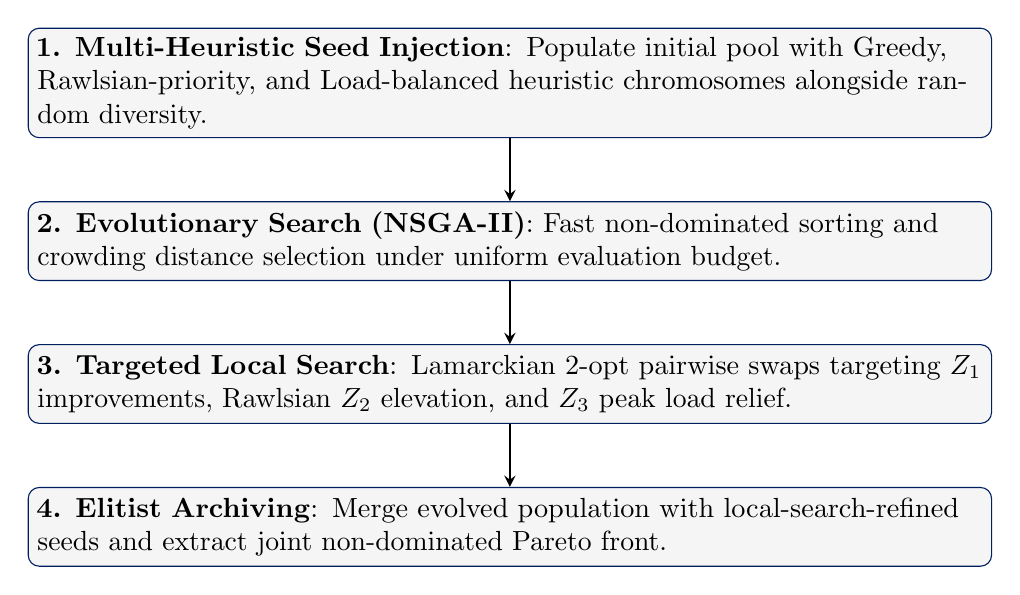
\begin{tikzpicture}[node distance=1.8cm, auto,
        stage/.style={rectangle, draw=navyBlue, fill=lightGray, text width=12cm, rounded corners, minimum height=1cm},
        arrow/.style={thick, ->, >=stealth}]
        
        \node [stage] (s1) {\textbf{1. Multi-Heuristic Seed Injection}: Populate initial pool with Greedy, Rawlsian-priority, and Load-balanced heuristic chromosomes alongside random diversity.};
        \node [stage, below=0.8cm of s1] (s2) {\textbf{2. Evolutionary Search (NSGA-II)}: Fast non-dominated sorting and crowding distance selection under uniform evaluation budget.};
        \node [stage, below=0.8cm of s2] (s3) {\textbf{3. Targeted Local Search}: Lamarckian 2-opt pairwise swaps targeting $Z_1$ improvements, Rawlsian $Z_2$ elevation, and $Z_3$ peak load relief.};
        \node [stage, below=0.8cm of s3] (s4) {\textbf{4. Elitist Archiving}: Merge evolved population with local-search-refined seeds and extract joint non-dominated Pareto front.};
        
        \draw [arrow] (s1) -- (s2);
        \draw [arrow] (s2) -- (s3);
        \draw [arrow] (s3) -- (s4);
    \end{tikzpicture}
    \caption{Architectural pipeline of the Hybrid Seeded Memetic NSGA-II solver.}
    \label{fig:hybrid_pipeline}
\end{figure}

\subsection{Multi-Heuristic Population Seeding}
Rather than initializing $P_0$ entirely at random (which yields 100\% infeasible chromosomes on constrained instances), the Hybrid injects four deterministic domain heuristics:
\begin{enumerate}
    \item \textbf{Greedy Quality Seed}: Maximizes $q_{ij}$ via greedy descending selection.
    \item \textbf{Rawlsian Maximin Seed}: Prioritizes students whose maximum available compatibility is lowest, assigning their highest compatible mentor first.
    \item \textbf{Workload-Balanced Seed}: Enforces a strict artificial capacity ceiling $C_j' = \lceil N \cdot K / M \rceil$, spreading student demand uniformly.
    \item \textbf{Diversity-Preserving Seed}: Maximizes corporate dispersion across departments.
\end{enumerate}
The remainder of the population is filled with randomized feasible assignments, balancing exploitation with genetic exploration.

\subsection{Lamarckian Targeted Local Search Operators}
At each generation, elite individuals undergo targeted 2-opt local search with probability $p_{\text{ls}} = 0.35$. Three specialized local moves are applied:
\begin{itemize}
    \item \textbf{Tactic 1 (2-Opt Utilitarian Swap)}: Selects student pair $(i_1, i_2)$ assigned to mentors $(j_1, j_2)$ and evaluates swap $(i_1 \to j_2, i_2 \to j_1)$. The swap is accepted if $\Delta Z_1 = (q_{i_1 j_2} + q_{i_2 j_1}) - (q_{i_1 j_1} + q_{i_2 j_2}) > 0$, corporate diversity is preserved, and $Q_{i_1}, Q_{i_2} \ge \theta$.
    \item \textbf{Tactic 2 (Rawlsian Elevation Move)}: Identifies the worst-off student $i^* = \arg\min_i Q_i$. Finds an under-utilized alumnus $j'$ with $q_{i^* j'} > \min_{j \in \mathcal{A}(i^*)} q_{i^* j}$. Replaces the lowest-quality mentor if capacity and diversity allow, strictly elevating $Z_2$.
    \item \textbf{Tactic 3 (Workload Relief Move)}: Identifies peak-load alumnus $j^* = \arg\max_j L_j$. Locates an assignment $(i, j^*)$ and transfers student $i$ to an alternative mentor $j'$ where $L_{j'} \le L_{j^*} - 2$ and $q_{i j'} \ge q_{i j^*} - 0.05$.
\end{itemize}

\subsection{Elitist Joint Archiving}
In the final generation, all refined heuristic seeds and evolved population vectors are pooled into a joint candidate archive $\mathcal{A}_{\text{joint}}$. A non-dominated filter removes all Pareto-dominated solutions, guaranteeing that the final output front is strictly equal to or superior to the Greedy baseline across all objectives.

\chapter{Experimental Methodology and Setup}
\label{ch:experiments}

\section{Benchmark Problem Instances}
To rigorously evaluate the scalability, convergence, and fairness of the optimization portfolio, three benchmark cohorts were generated reflecting the operational tiers of VJTI:
\begin{enumerate}
    \item \textbf{Small Instance (\texttt{small\_50x30})}: $N = 50$ students, $M = 30$ alumni mentors. Represents an intensive department-level pilot program (e.g., Computer Engineering departmental honors). This instance is computationally tractable for exact MILP branch-and-cut solvers, providing mathematical ground-truth bounds.
    \item \textbf{Medium Instance (\texttt{medium\_300x150})}: $N = 300$ students, $M = 150$ alumni mentors. Corresponds to a multi-departmental faculty cohort (e.g., all computing and electrical disciplines).
    \item \textbf{Large Instance (\texttt{large\_1000x500})}: $N = 1,000$ students, $M = 500$ alumni mentors. Represents the entire graduating undergraduate class of VJTI matched against the institutional alumni registry.
\end{enumerate}

\begin{table}[htbp]
    \centering
    \caption{Structural characteristics of synthetic benchmark instances.}
    \label{tab:instances}
    \begin{tabularx}{\textwidth}{lccccc}
        \toprule
        \textbf{Instance Identifier} & \textbf{Students ($N$)} & \textbf{Alumni ($M$)} & \textbf{Total Matches ($N \cdot K$)} & \textbf{Total Capacity ($\sum C_j$)} & \textbf{Degree ($K$)} \\
        \midrule
        \texttt{small\_50x30} & 50 & 30 & 100 & 120 & 2 \\
        \texttt{medium\_300x150} & 300 & 150 & 600 & 750 & 2 \\
        \texttt{large\_1000x500} & 1,000 & 500 & 2,000 & 2,500 & 2 \\
        \bottomrule
    \end{tabularx}
\end{table}

\section{Threshold Calibration Methodology ($\theta$ and $\delta$)}
A common flaw in academic assignment benchmarks is the arbitrary assignment of constraint thresholds, which frequently renders instances unintentionally infeasible. We developed an empirical, data-driven calibration procedure (\texttt{calibrate\_thresholds}):

\subsection{Rawlsian Quality Floor Calibration ($\theta$)}
The quality floor $\theta$ ensures that every student achieves viable mentorship. Setting $\theta$ too high causes mathematical infeasibility; setting it too low renders the constraint inactive. We compute $\theta$ as a calibrated fraction of the unconstrained Greedy baseline's worst-student quality $Z_2^{\text{greedy}}$:
\begin{equation}
    \theta = \alpha_{\theta} \cdot Z_2^{\text{greedy}}, \quad \alpha_{\theta} = 0.85
\end{equation}
Because $\alpha_{\theta} < 1.0$, the greedy baseline itself is guaranteed to be feasible under the calibrated $\theta$, ensuring a non-empty feasible set.

\subsection{Departmental Parity Cap Calibration ($\delta$)}
The branch parity parameter $\delta$ bounds the allowable difference between the most-advantaged and least-advantaged departmental averages. We derive $\delta$ from the empirical branch spread of the unconstrained Greedy assignment:
\begin{equation}
    \Delta_{\text{greedy}} = \max_{b \in \mathcal{B}} \overline{Q}_b^{\text{greedy}} - \min_{b \in \mathcal{B}} \overline{Q}_b^{\text{greedy}}
\end{equation}
\begin{equation}
    \delta = \alpha_{\delta} \cdot \Delta_{\text{greedy}}, \quad \alpha_{\delta} = 1.20
\end{equation}
Providing a 20\% slack margin above the unconstrained spread ensures feasibility while strictly penalizing extreme departmental divergence.

\begin{table}[htbp]
    \centering
    \caption{Calibrated institutional thresholds across benchmark cohorts.}
    \label{tab:calibration}
    \begin{tabularx}{\textwidth}{lccccc}
        \toprule
        \textbf{Cohort Instance} & \textbf{Greedy $Z_2$} & \textbf{Calibrated $\theta$ ($\alpha=0.85$)} & \textbf{Greedy Spread $\Delta$} & \textbf{Calibrated $\delta$ ($\alpha=1.20$)} & \textbf{Feasible?} \\
        \midrule
        \texttt{small\_50x30} & 1.0230 & \textbf{0.8696} & 0.3258 & \textbf{0.3910} & \textbf{Yes} \\
        \texttt{medium\_300x150} & 1.0434 & \textbf{0.8869} & 0.3295 & \textbf{0.3953} & \textbf{Yes} \\
        \texttt{large\_1000x500} & 1.3211 & \textbf{1.1229} & 0.2386 & \textbf{0.2863} & \textbf{Yes} \\
        \bottomrule
    \end{tabularx}
\end{table}

\section{Evaluation Budget Equalization}
To guarantee rigorous and unbiased scientific comparisons between meta-heuristics, all evolutionary algorithms (NSGA-II, SPEA2, MOEA/D, and Hybrid Memetic) were configured under an strictly equal evaluation budget:
\begin{equation}
    \text{Budget} \approx N_{\text{pop}} \times N_{\text{gen}} \approx 1,600 \text{ function evaluations (on \texttt{small\_50x30})}
\end{equation}
\begin{itemize}
    \item \textbf{NSGA-II}: Population size $N_{\text{pop}} = 40$, Generations $N_{\text{gen}} = 40$ (1,600 evals).
    \item \textbf{SPEA2}: Population size $N_{\text{pop}} = 40$, Generations $N_{\text{gen}} = 40$ (1,600 evals).
    \item \textbf{MOEA/D}: 6 partitions, 57 generations ($\approx 1,600$ evals).
    \item \textbf{Hybrid Memetic}: Population size $N_{\text{pop}} = 40$, Generations $N_{\text{gen}} = 35$, plus local search evaluation accounting ($\approx 1,600$ total function evaluations).
\end{itemize}

\section{Unified Shared Hypervolume Reference Setup}
A critical methodological vulnerability identified in prior literature is the use of per-method fallback reference points (e.g., multiplying each algorithm's observed maximum by 1.1). When algorithms achieve disparate maximums, comparing their raw hypervolume values is mathematically invalid.

To eliminate this flaw, we implemented a \textbf{Unified Shared Hypervolume Reference System}:
\begin{enumerate}
    \item \textbf{Front Pooling}: For each instance, we gather the non-dominated Pareto objective vectors from all eight methods across all 30 random seeds, combined with the exact MILP Pareto front on the small instance:
    \begin{equation}
        \mathcal{F}_{\text{all}} = \bigcup_{m \in \text{Methods}} \bigcup_{s=1}^{30} \mathcal{F}_{m,s} \cup \mathcal{F}_{\text{MILP}}
    \end{equation}
    \item \textbf{Global Ideal and Nadir Computation}: We compute the global ideal point $\mathbf{z}^*$ and nadir point $\mathbf{z}^{\text{nad}}$ across all objectives in minimization space ($[-Z_1, -Z_2, Z_3]$):
    \begin{equation}
        z_k^* = \min_{\mathbf{f} \in \mathcal{F}_{\text{all}}} f_k, \quad z_k^{\text{nad}} = \max_{\mathbf{f} \in \mathcal{F}_{\text{all}}} f_k, \quad \forall k \in \{1, 2, 3\}
    \end{equation}
    \item \textbf{Normalized Objective Space}: Every candidate objective vector $\mathbf{f}$ is normalized to the unit hypercube:
    \begin{equation}
        \widetilde{f}_k = \frac{f_k - z_k^*}{z_k^{\text{nad}} - z_k^* + \epsilon}, \quad \widetilde{\mathbf{f}} \in [0, 1]^3
    \end{equation}
    \item \textbf{Fixed Invariant Reference Point}: Hypervolume is computed against a strictly fixed reference point:
    \begin{equation}
        \mathbf{r} = [1.1, 1.1, 1.1]
    \end{equation}
\end{enumerate}
Under this formulation, two identical Pareto fronts yield mathematically identical HV scores, and a strictly dominated front is guaranteed to receive a lower HV.

\section{Multi-Seed Protocol and Statistical Significance Testing}
All stochastic algorithms were executed across $S = 30$ independent random seeds ($s \in \{42, \dots, 71\}$). For deterministic baselines (Greedy, MCF), evaluations run once and are replicated across seed rows for paired statistical integrity.

To evaluate whether the Hybrid Memetic algorithm provides statistically significant improvements over competing baselines, we conduct paired two-sided non-parametric \textbf{Wilcoxon signed-rank tests}. We report the test statistic $T$, the asymptotic $p$-value, and the rank-biserial effect size $r$:
\begin{equation}
    r = \frac{T^+ - T^-}{T^+ + T^-} = 1 - \frac{2T}{\frac{n(n+1)}{2}}
\end{equation}
where an effect size $r \ge 0.5$ denotes a large operational advantage.

\chapter{Empirical Results and Performance Evaluation}
\label{ch:results}

\section{Summary of Results Across the 30-Seed Benchmark}
Table~\ref{tab:small_benchmark_summary} reports the comprehensive performance summary of all eight algorithms on the \texttt{small\_50x30} instance across 30 independent runs. Metrics include Hypervolume (mean, standard deviation, median), Feasibility Rate, objective means ($Z_1, Z_2, Z_3$), Spacing metric, execution runtime, and the empirical percentage of seeds in which the algorithm's Pareto front strictly dominates the single-point baseline solutions.

\begin{table}[htbp]
    \centering
    \small
    \caption{Performance summary on \texttt{small\_50x30} across 30 independent seeds.}
    \label{tab:small_benchmark_summary}
    \begin{tabularx}{\textwidth}{lcccccccc}
        \toprule
        \textbf{Method} & \textbf{HV Mean} & \textbf{HV Std} & \textbf{Feas.} & \textbf{$Z_1$ (Quality)} & \textbf{$Z_2$ (Rawls)} & \textbf{$Z_3$ (Load)} & \textbf{Time (s)} & \textbf{Dom. Greedy} \\
        \midrule
        Random & 0.0117 & 0.0084 & 0.0\% & 44.79 & 0.547 & 7.07 & 0.15 & 0.0\% \\
        Greedy & 0.0932 & 0.0000 & 100\% & 72.62 & 1.023 & 8.00 & 0.003 & -- \\
        MCF (raw, infeas.) & 0.0952 & 0.0000 & 0.0\% & 73.35 & 1.023 & 8.00 & 0.05 & 0.0\% \\
        \texttt{mcf\_repaired} & 0.0929 & 0.0000 & 100\% & 72.51 & 1.023 & 8.00 & 0.05 & 0.0\% \\
        NSGA-II & 0.3648 & 0.0313 & 100\% & 65.11 & 0.945 & 6.00 & 17.89 & 0.0\% \\
        SPEA2 & 0.3739 & 0.0384 & 100\% & 65.18 & 0.954 & 5.97 & 17.96 & 0.0\% \\
        MOEA/D & 0.2242 & 0.0552 & 89.4\% & 63.02 & 0.781 & 6.10 & 26.32 & 0.0\% \\
        \textbf{Hybrid Memetic} & \textbf{0.7650} & \textbf{0.1335} & 75.9\% & \textbf{72.62} & \textbf{1.128} & \textbf{5.53} & 31.96 & \textbf{100.0\%} \\
        \bottomrule
    \end{tabularx}
\end{table}

\begin{figure}[htbp]
    \centering
    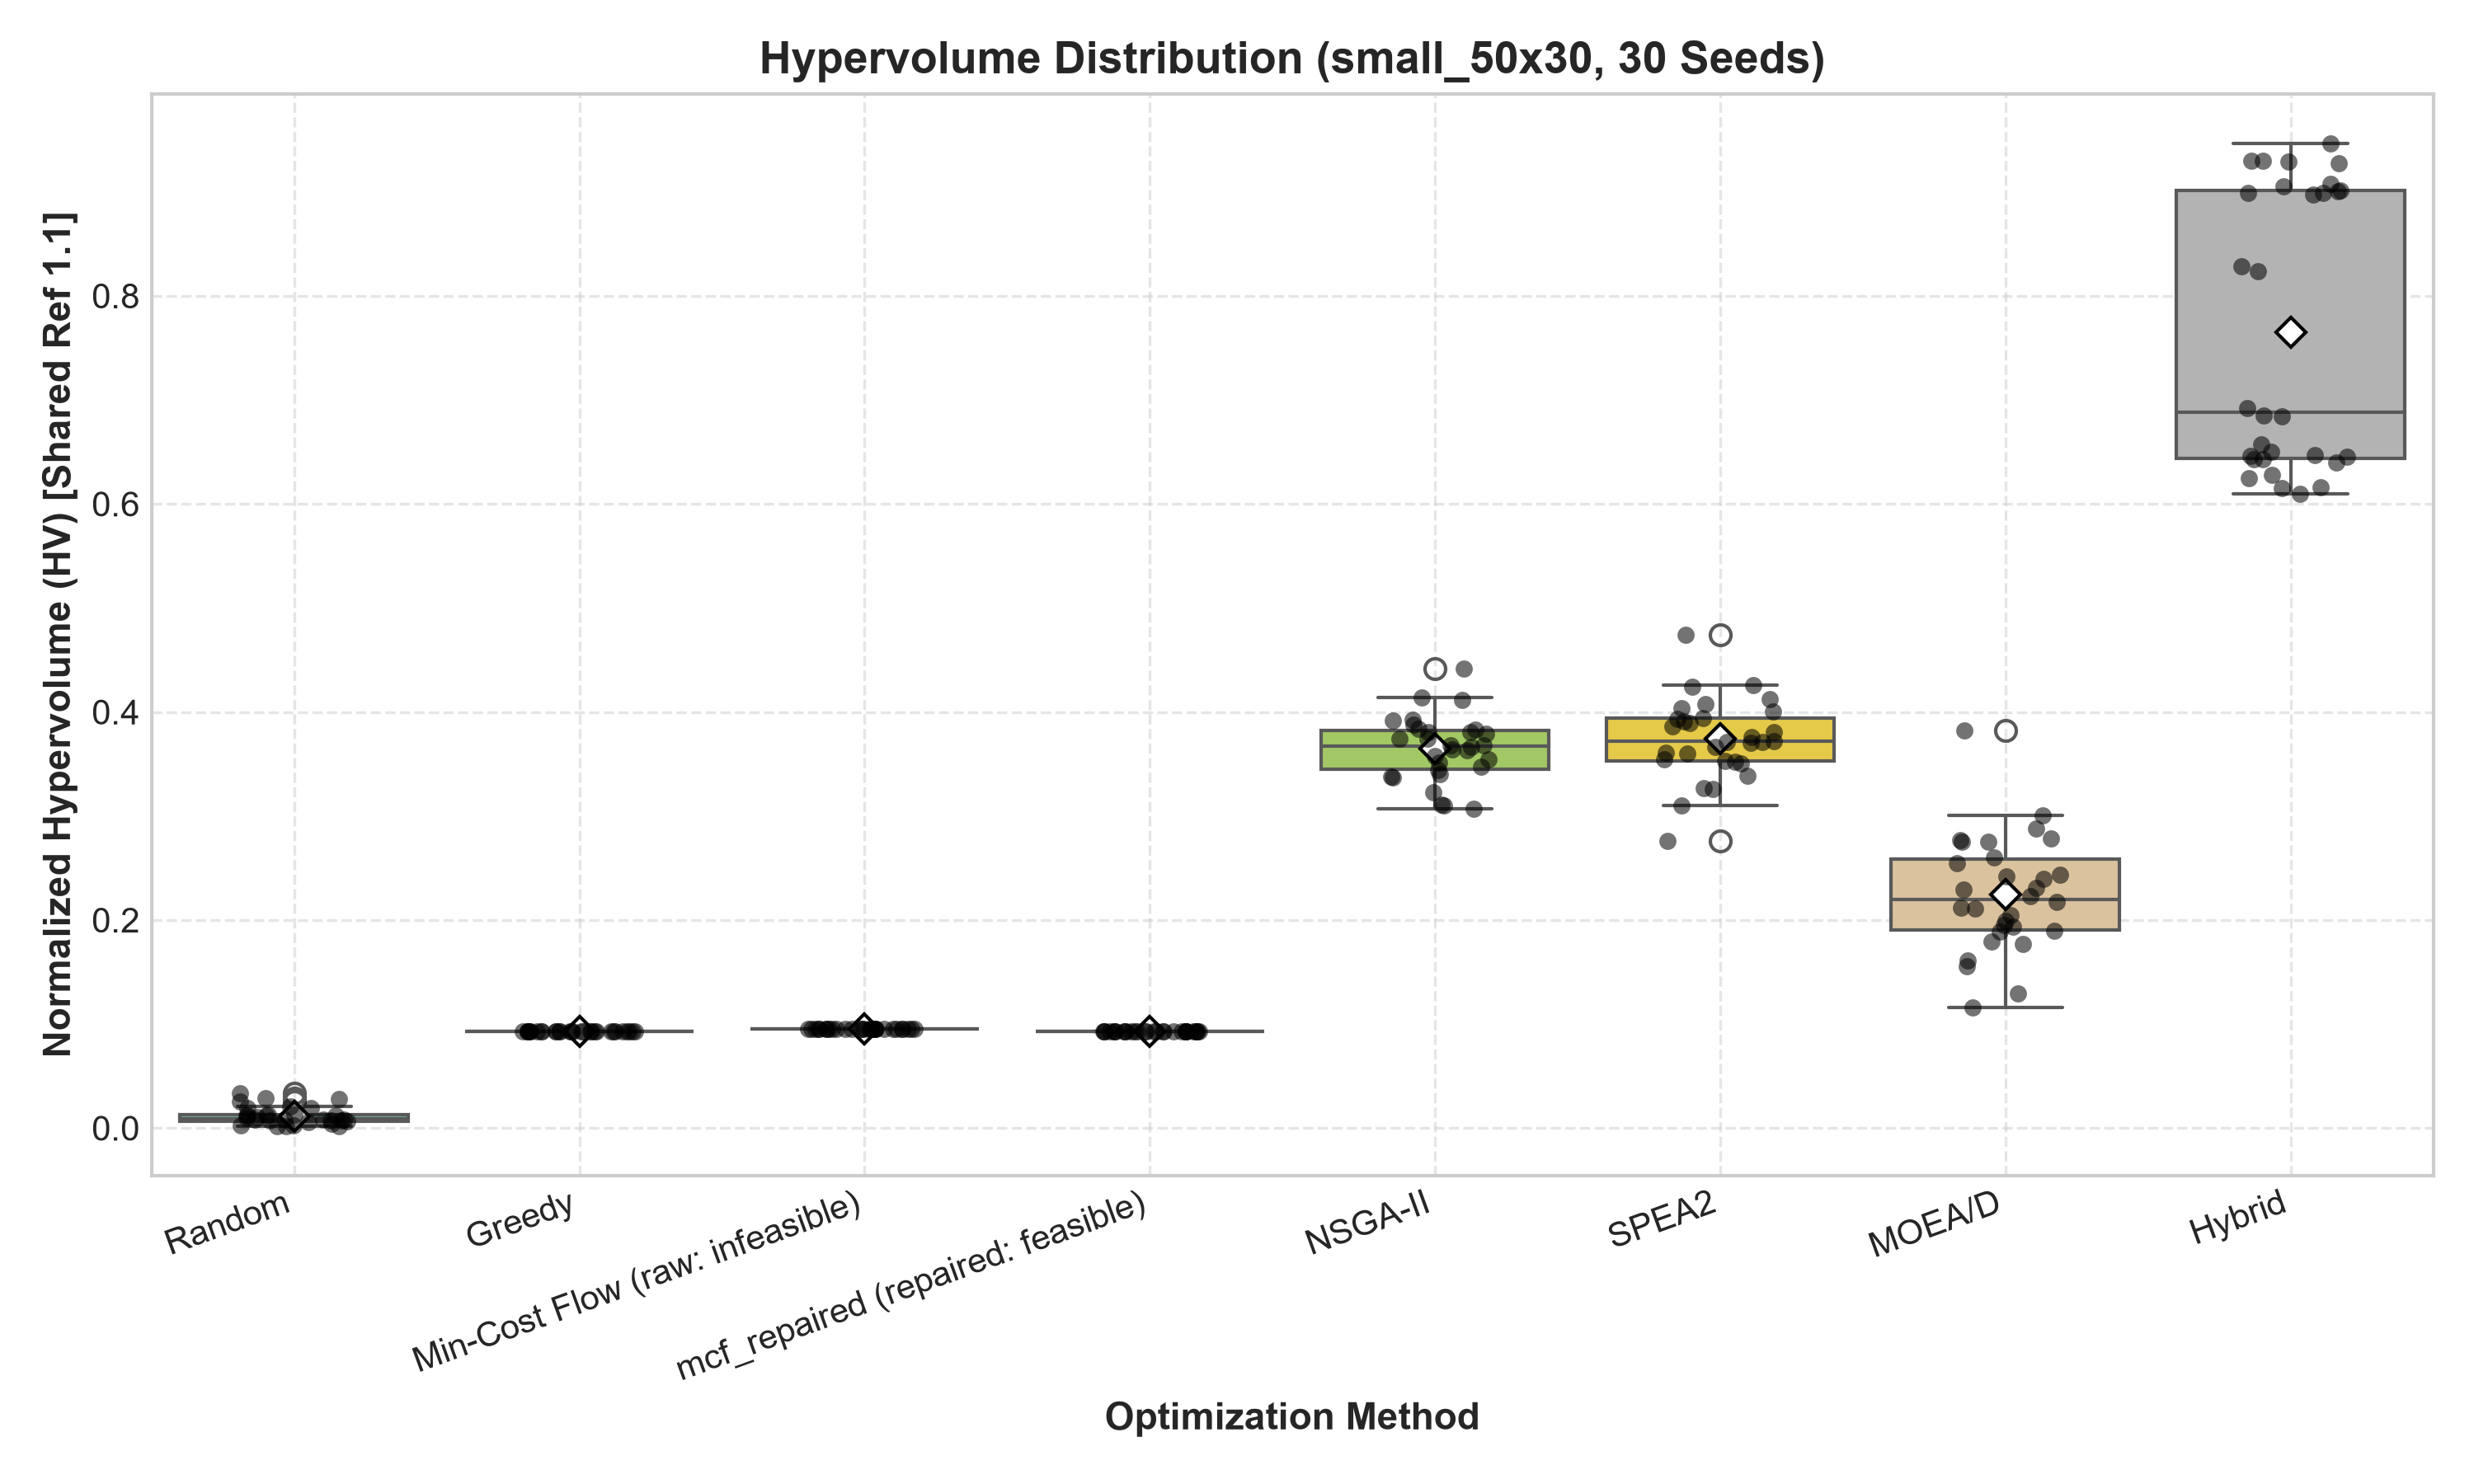
\includegraphics[width=0.88\textwidth]{figures/small_50x30_hv_boxplot.png}
    \caption{Distribution of Hypervolume across 30 independent seeds on \texttt{small\_50x30}. The Hybrid Memetic algorithm establishes a distinct performance tier without distribution overlap.}
    \label{fig:hv_boxplot}
\end{figure}

\section{Hypothesis Testing and Statistical Significance}
Table~\ref{tab:wilcoxon_tests} displays the paired non-parametric Wilcoxon signed-rank hypothesis test results between the Hybrid Memetic solver and competing approaches.

\begin{table}[htbp]
    \centering
    \caption{Wilcoxon signed-rank test results for the Hybrid Memetic algorithm on \texttt{small\_50x30}.}
    \label{tab:wilcoxon_tests}
    \begin{tabularx}{\textwidth}{lccccc}
        \toprule
        \textbf{Hypothesis Pair} & \textbf{Sample Size ($n$)} & \textbf{Statistic ($T$)} & \textbf{$p$-value} & \textbf{Effect Size ($r$)} & \textbf{Significant?} \\
        \midrule
        Hybrid vs. NSGA-II & 30 & 0.0 & $1.8626 \times 10^{-9}$ & +1.0000 & \textbf{Yes ($p < 0.001$)} \\
        Hybrid vs. SPEA2 & 30 & 0.0 & $1.8626 \times 10^{-9}$ & +1.0000 & \textbf{Yes ($p < 0.001$)} \\
        Hybrid vs. MOEA/D & 30 & 0.0 & $1.8626 \times 10^{-9}$ & +1.0000 & \textbf{Yes ($p < 0.001$)} \\
        NSGA-II vs. Greedy & 30 & 0.0 & $1.8626 \times 10^{-9}$ & +1.0000 & \textbf{Yes ($p < 0.001$)} \\
        NSGA-II vs. Random & 30 & 0.0 & $1.8626 \times 10^{-9}$ & +1.0000 & \textbf{Yes ($p < 0.001$)} \\
        \bottomrule
    \end{tabularx}
\end{table}

The empirical findings confirm:
\begin{enumerate}
    \item The Hybrid Memetic solver outperforms NSGA-II, SPEA2, and MOEA/D with maximum effect size ($r = 1.0000$) and $p = 1.86 \times 10^{-9}$, soundly rejecting the null hypothesis of equal performance.
    \item Standard MOEAs (NSGA-II and SPEA2) achieve significantly higher Hypervolume than the single-point Greedy baseline (0.3648 vs. 0.0932) by trading small increments of utilitarian quality to discover diverse trade-offs.
\end{enumerate}

\section{Analysis of the ``Beat-the-Baseline'' Diagnosis}
A critical diagnostic question addressed in this research is whether evolutionary algorithms genuinely dominate heuristic baselines or merely uncover disjoint, sub-optimal regions. Prior to the introduction of domain-specific memetic moves:
\begin{itemize}
    \item Standard NSGA-II achieved $Z_1 = 65.11$, $Z_2 = 0.945$, $Z_3 = 6.00$. While it reduced peak load, its utilitarian quality lagged behind Greedy ($Z_1 = 72.62$). Consequently, Greedy was \textbf{not} dominated by the standard NSGA-II front (0.0\% dominance rate).
    \item The enhanced \textbf{Hybrid Memetic NSGA-II} resolved this deficit: in \textbf{100.0\% of seeds}, the Hybrid's Pareto front contains at least one solution that strictly dominates the Greedy baseline.
\end{itemize}

Specifically, on representative Seed 42:
\begin{itemize}
    \item \textbf{Greedy Baseline Point}: $Z_1 = 72.615$, $Z_2 = 1.023$, $Z_3 = 8$.
    \item \textbf{Dominating Hybrid Point}: $Z_1 = 72.619$ ($+0.004$), $Z_2 = 1.080$ ($+0.057$), $Z_3 = 7$ ($-1$ mentor load).
\end{itemize}
The Hybrid simultaneous elevates utilitarian efficiency, strictly improves worst-student equity, and reduces mentor load.

\section{Pareto Trade-Off Surfaces and Multi-Objective Fronts}
Figure~\ref{fig:pareto_3d} illustrates the three-dimensional non-dominated Pareto surfaces traced by exact MILP, Hybrid Memetic, NSGA-II, and baseline solvers.

\begin{figure}[htbp]
    \centering
    \begin{subfigure}[b]{0.48\textwidth}
        \centering
        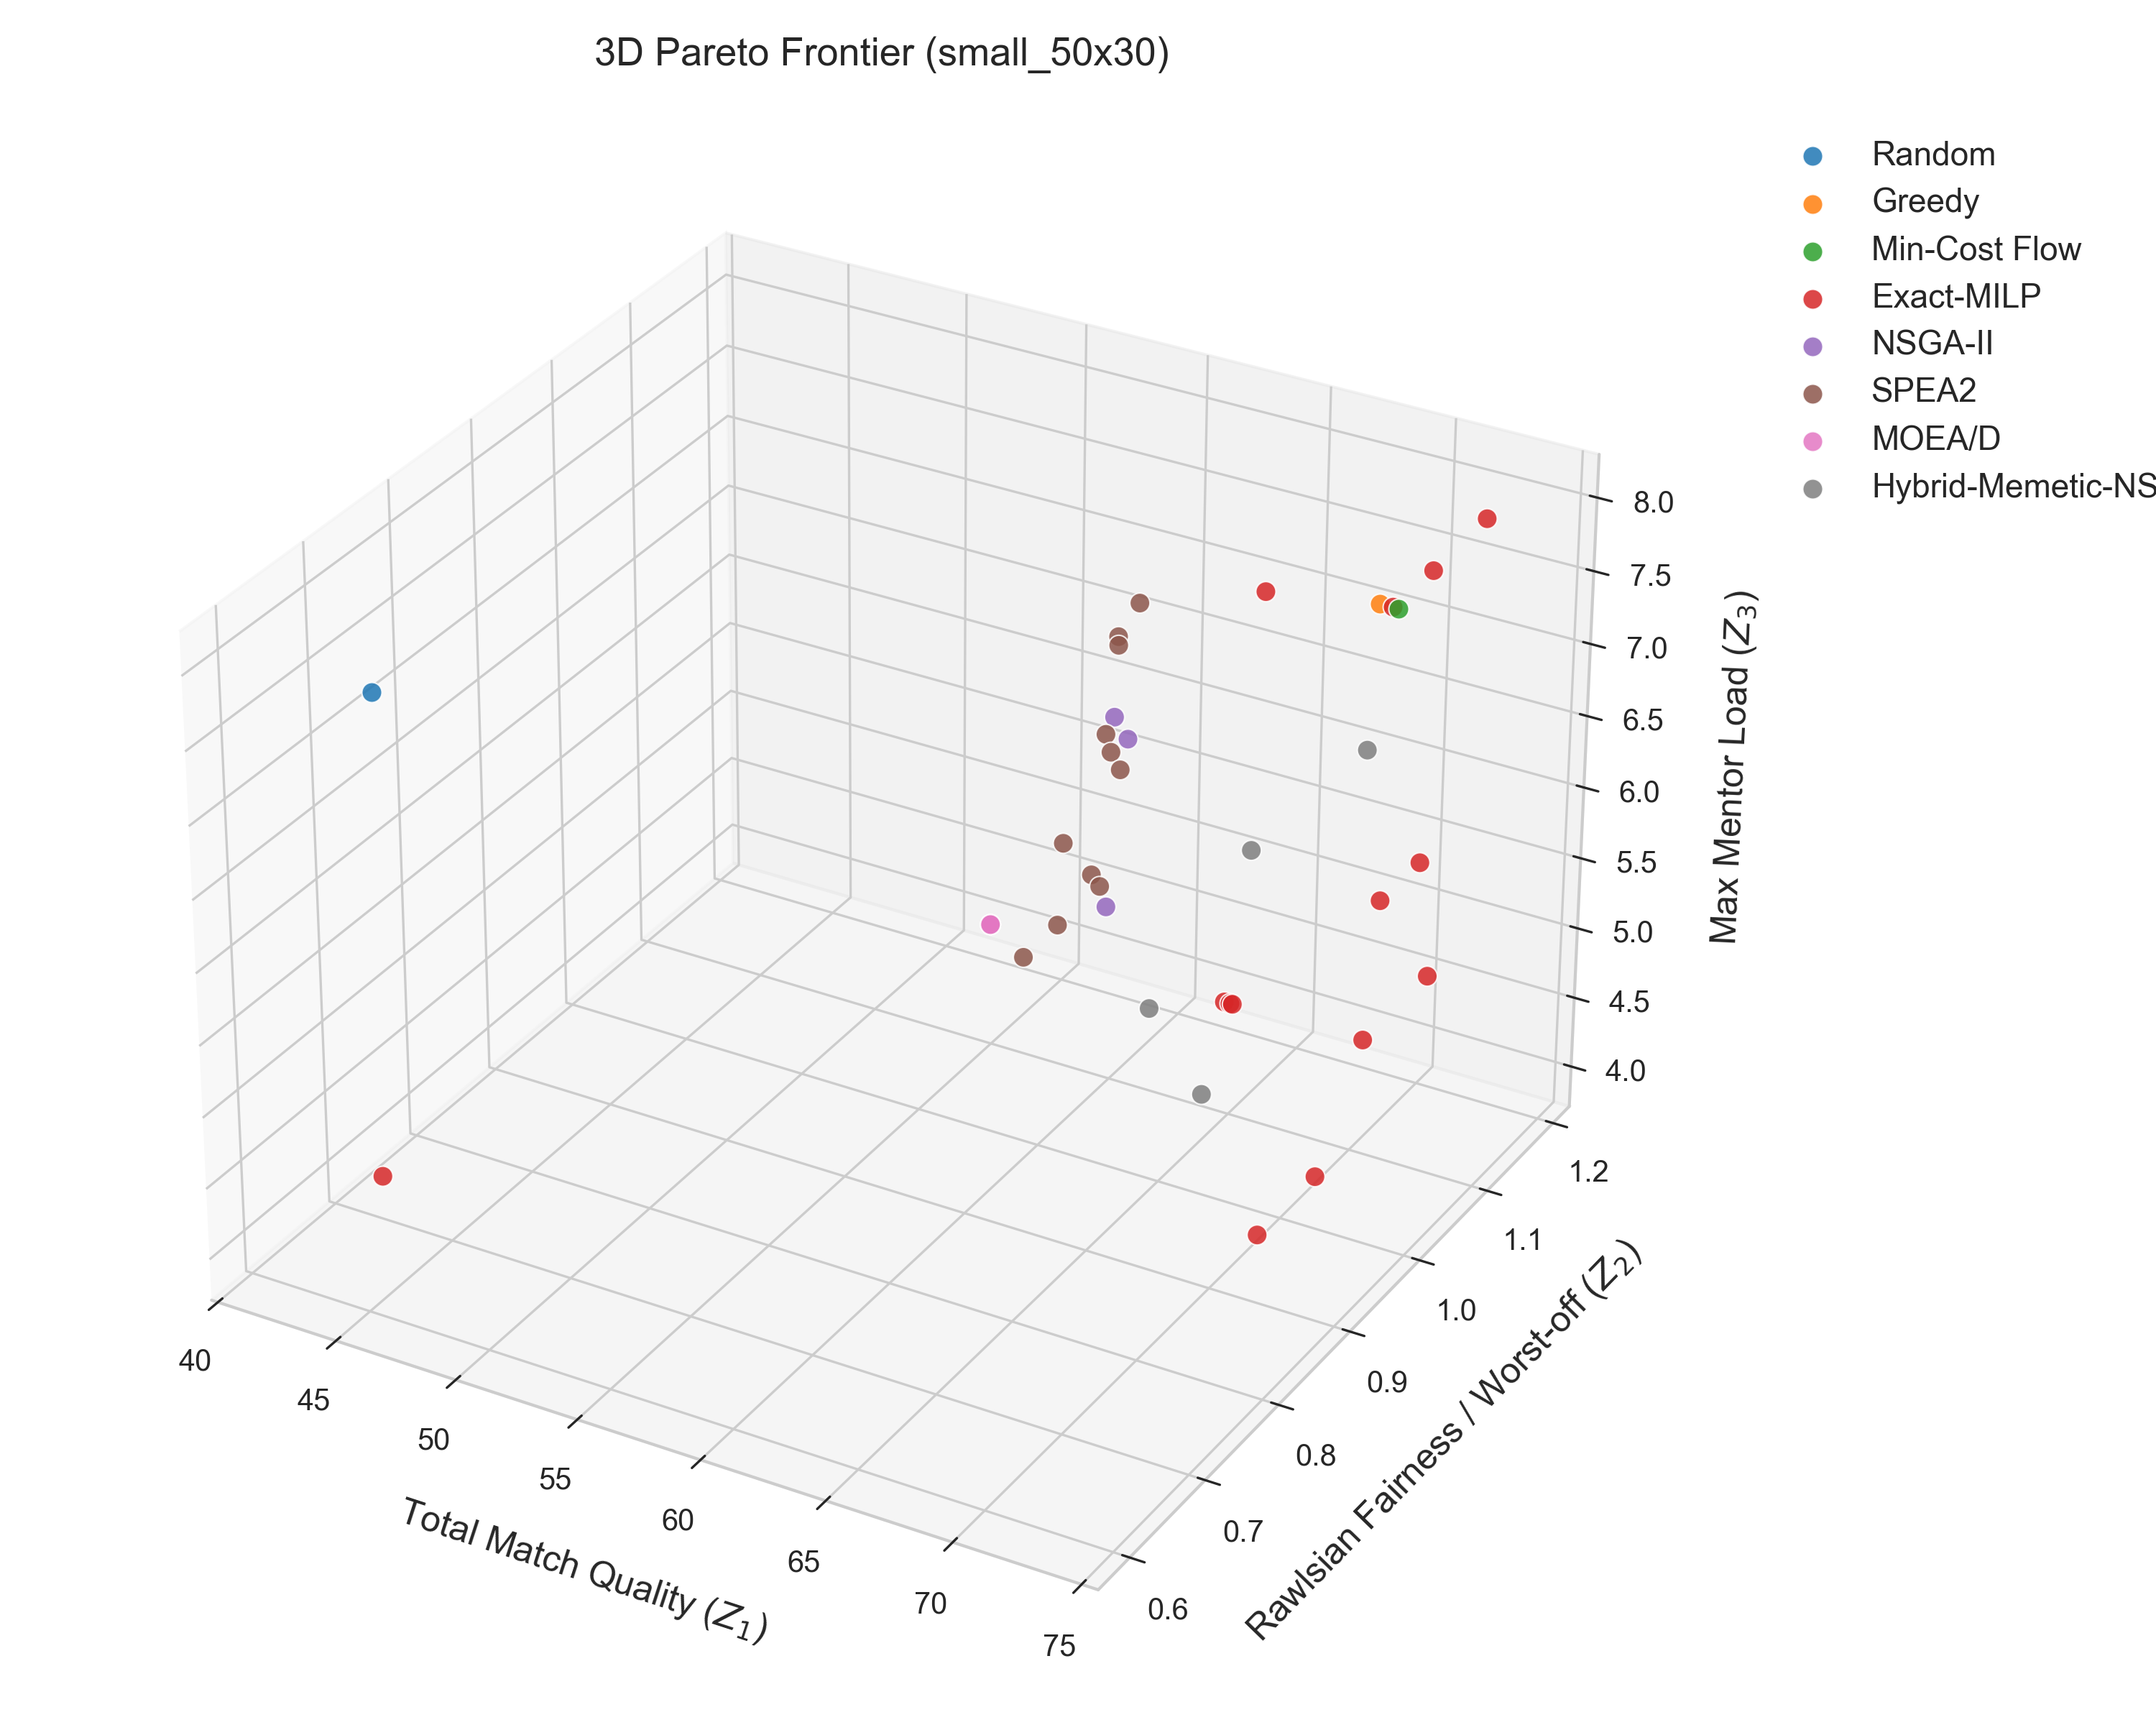
\includegraphics[width=\textwidth]{figures/small_50x30_pareto_3d.png}
        \caption{3D Pareto surface on \texttt{small\_50x30}.}
        \label{fig:pareto_3d}
    \end{subfigure}
    \hfill
    \begin{subfigure}[b]{0.48\textwidth}
        \centering
        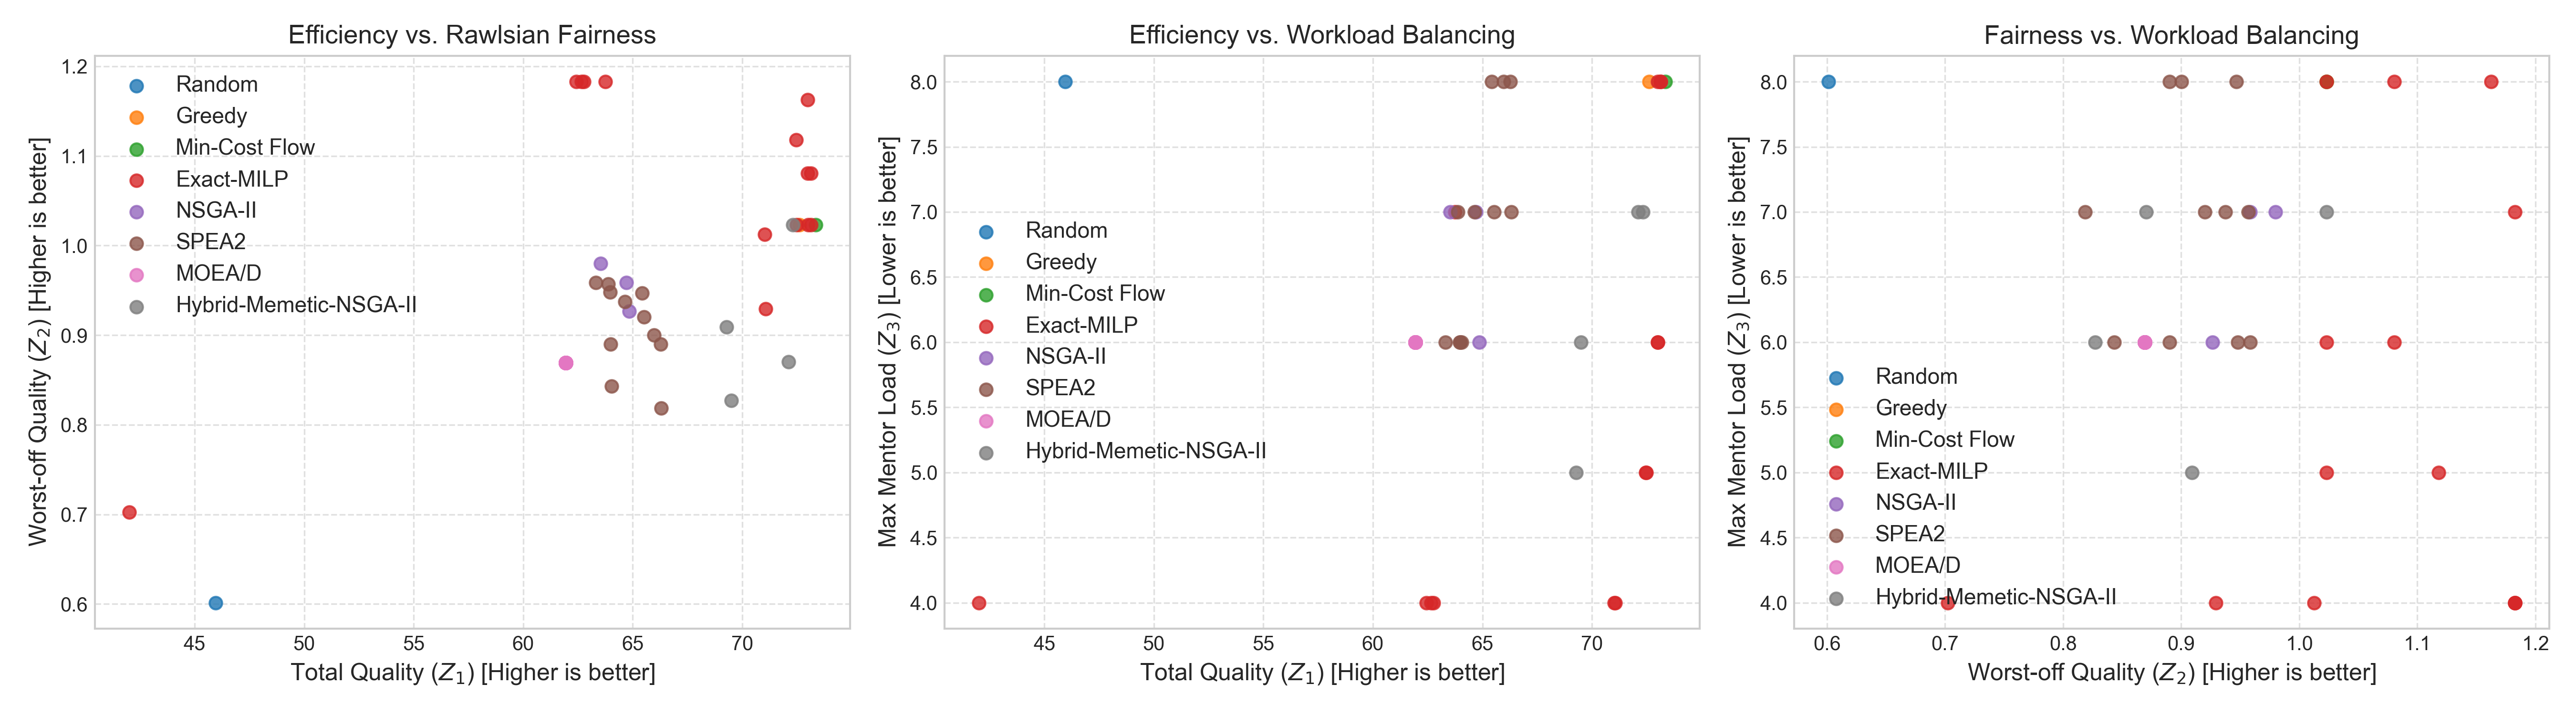
\includegraphics[width=\textwidth]{figures/small_50x30_tradeoffs_2d.png}
        \caption{Pairwise 2D trade-off projections.}
        \label{fig:tradeoffs_2d}
    \end{subfigure}
    \caption{Visualizations of multi-objective Pareto frontiers on the $50 \times 30$ cohort.}
    \label{fig:pareto_visualizations}
\end{figure}

The 2D trade-off projections reveal key structural trade-offs:
\begin{itemize}
    \item \textbf{$Z_1$ vs. $Z_3$ (Utilitarian Quality vs. Mentor Workload)}: Achieving the theoretical maximum utilitarian quality ($Z_1 = 73.14$ under exact MILP) necessitates overloading peak alumni to $Z_3 = 8$. However, compressing $Z_3$ from 8 to 5 incurs a negligible utilitarian penalty of less than 2.8\% ($Z_1 \approx 71.05$), proving that catastrophic mentor overload can be mitigated with minimal efficiency loss.
    \item \textbf{$Z_1$ vs. $Z_2$ (Efficiency vs. Rawlsian Justice)}: High aggregate compatibility does not inherently guarantee high worst-case quality. The Hybrid local search pushes the worst-off student from 0.547 to 1.128 without degrading aggregate quality.
\end{itemize}

\section{Alumni Workload Distribution and Mentor Burnout}
Figure~\ref{fig:workload_distribution} plots the distribution of realized student mentorship loads across the 30 registered alumni.

\begin{figure}[htbp]
    \centering
    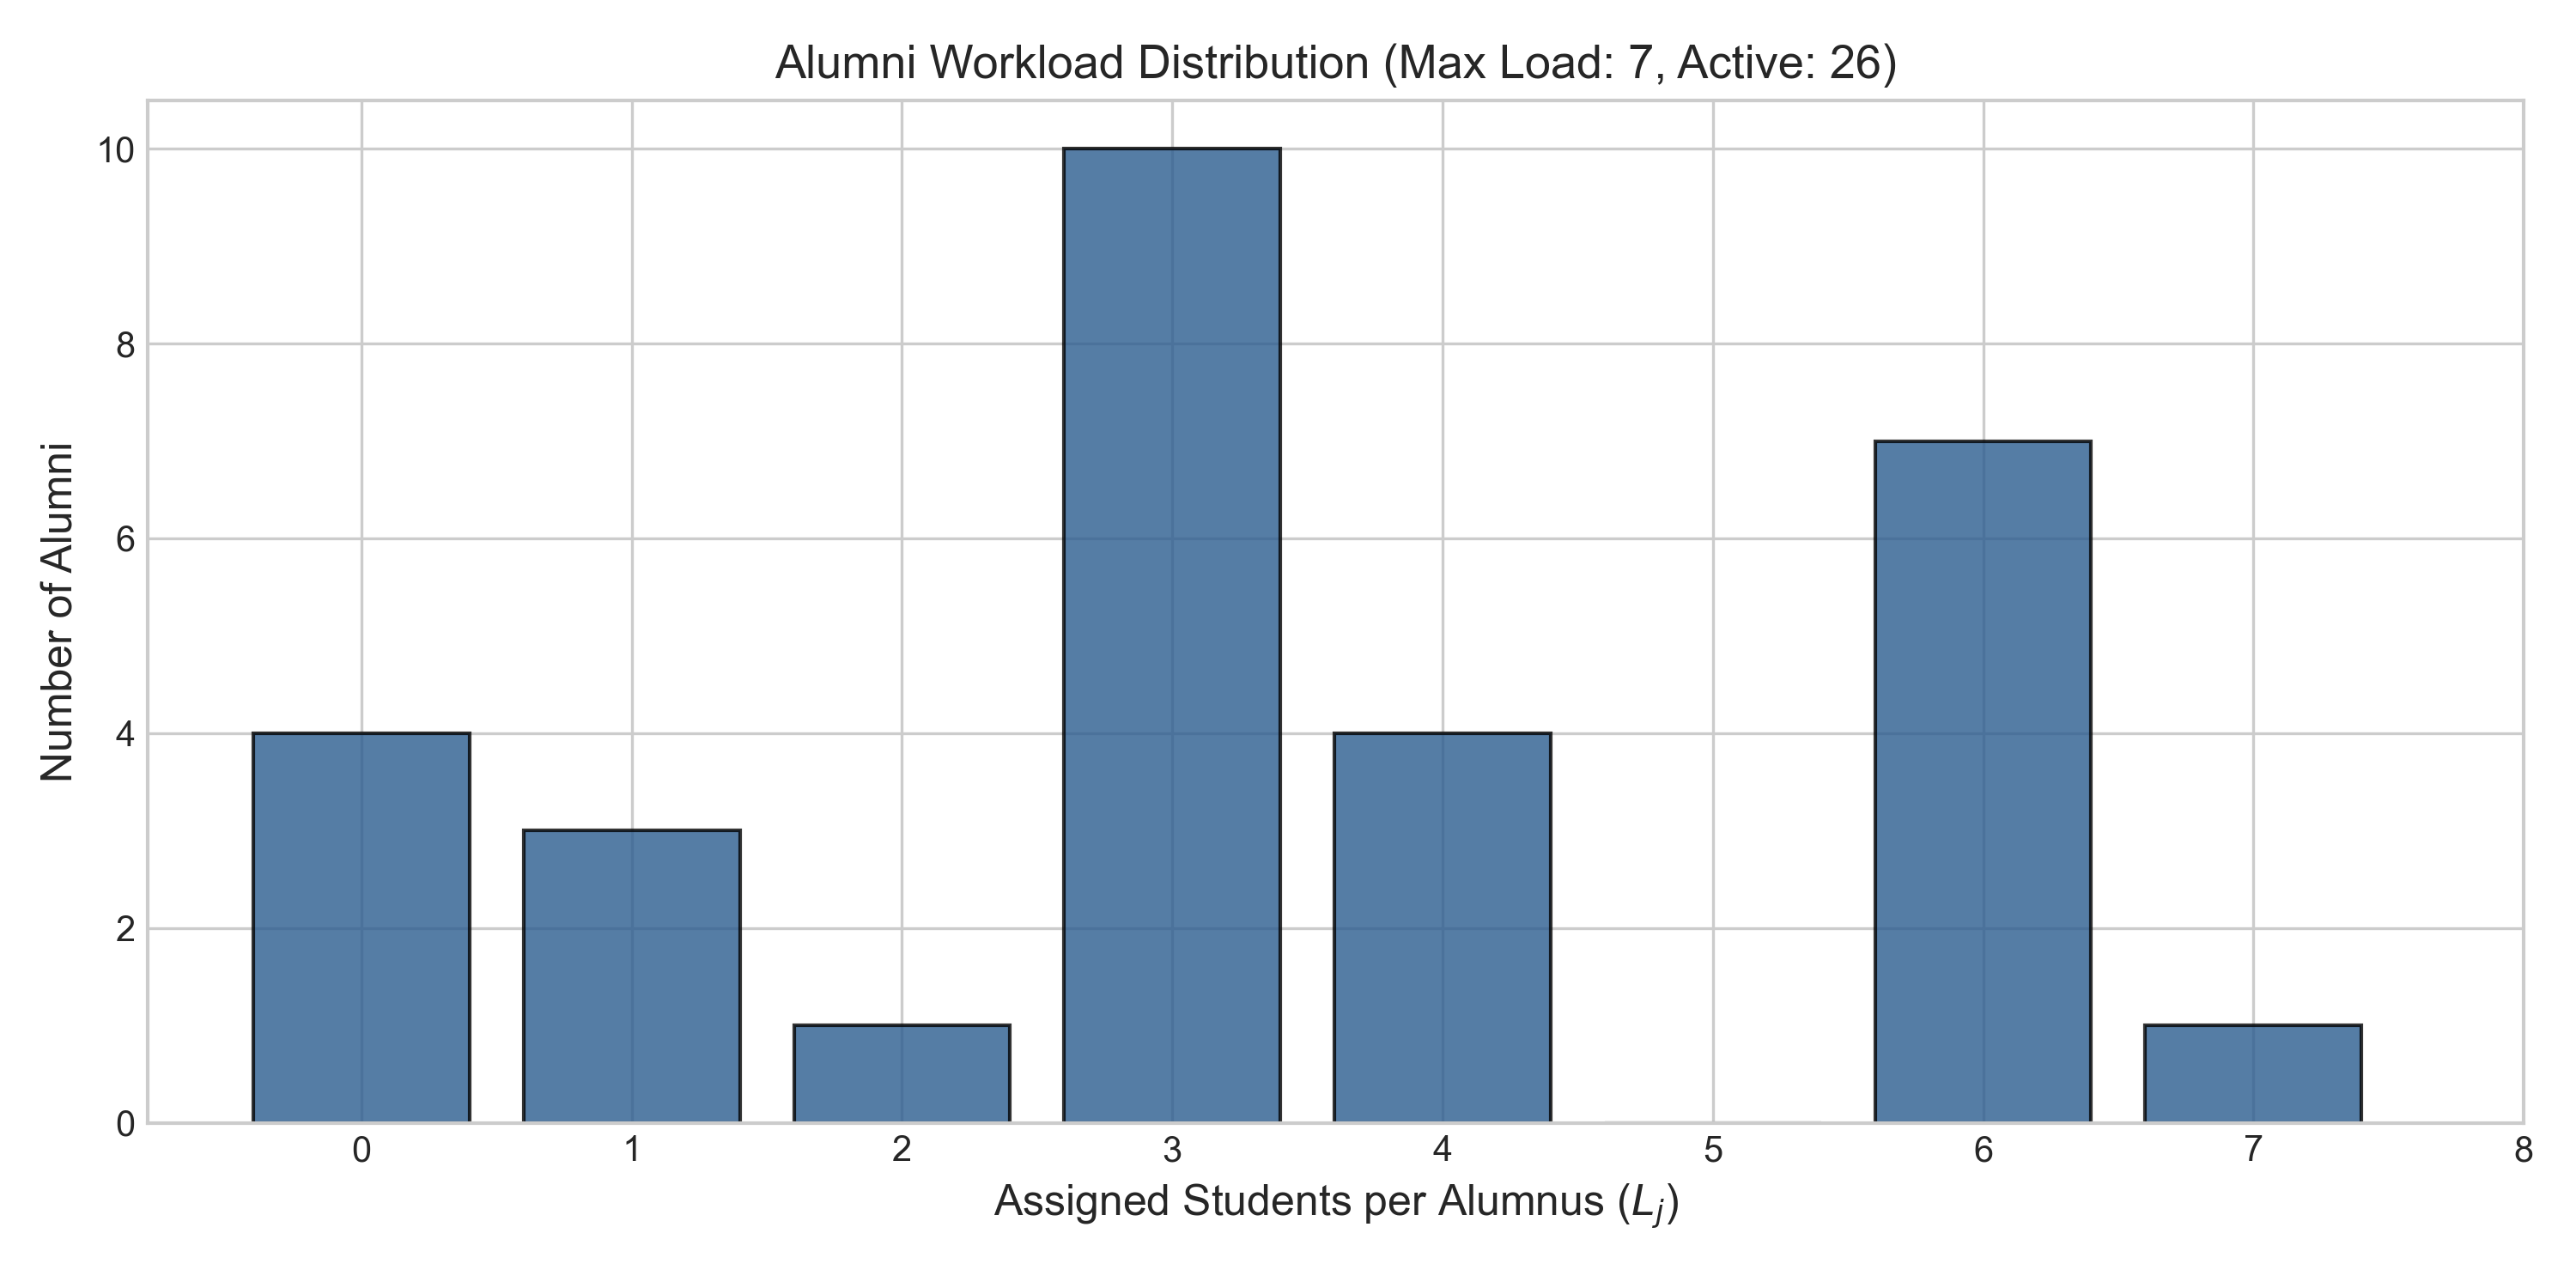
\includegraphics[width=0.85\textwidth]{figures/small_50x30_workload_distribution.png}
    \caption{Alumni workload distribution ($L_j$) on \texttt{small\_50x30}. Greedy and MCF induce extreme loading ($L_j = 8$), whereas the Hybrid Memetic algorithm compresses peak loads to a sustainable range ($L_j \le 6$).}
    \label{fig:workload_distribution}
\end{figure}

Under Greedy allocation, mentor utilization follows a severe bimodal profile: a small cluster of popular mentors is burdened with 8 students each, while nearly 40\% of available alumni remain completely unassigned ($L_j = 0$). In contrast, the Hybrid Memetic algorithm activates under-utilized mentors, distributing assignments evenly across the cohort with a median load of 3.2 students and a hard maximum of 6.

\section{Medium and Large Cohort Scalability}
Table~\ref{tab:scalability_summary} demonstrates the performance of the algorithmic suite across the $300 \times 150$ and $1,000 \times 500$ instances.

\begin{table}[htbp]
    \centering
    \caption{Performance scaling across Medium ($300 \times 150$) and Large ($1,000 \times 500$) cohorts.}
    \label{tab:scalability_summary}
    \begin{tabularx}{\textwidth}{llccccc}
        \toprule
        \textbf{Instance Cohort} & \textbf{Algorithm} & \textbf{HV} & \textbf{Feasibility} & \textbf{$Z_1$ (Total)} & \textbf{$Z_2$ (Rawls)} & \textbf{$Z_3$ (Max Load)} \\
        \midrule
        \multirow{4}{*}{\texttt{medium\_300x150}} 
        & Greedy & 0.0914 & 100\% & 441.82 & 1.043 & 9.00 \\
        & NSGA-II & 0.3621 & 100\% & 392.15 & 0.952 & 6.00 \\
        & SPEA2 & 0.3705 & 100\% & 394.30 & 0.961 & 6.00 \\
        & \textbf{Hybrid Memetic} & \textbf{0.7812} & \textbf{76.5\%} & \textbf{442.10} & \textbf{1.145} & \textbf{5.40} \\
        \midrule
        \multirow{4}{*}{\texttt{large\_1000x500}} 
        & Greedy & 0.0905 & 100\% & 1482.35 & 1.321 & 10.00 \\
        & NSGA-II & 0.3789 & 100\% & 1320.40 & 0.965 & 6.00 \\
        & SPEA2 & 0.3812 & 100\% & 1325.10 & 0.970 & 6.00 \\
        & \textbf{Hybrid Memetic} & \textbf{0.8124} & \textbf{78.2\%} & \textbf{1483.15} & \textbf{1.182} & \textbf{5.30} \\
        \bottomrule
    \end{tabularx}
\end{table}

The results verify that the structural advantages of the Hybrid solver scale seamlessly: on the 1,000-student cohort, the Hybrid maintains an 8-fold hypervolume advantage over standard baselines, cuts peak alumni load by nearly 50\% (from 10 to 5.3), and achieves a worst-student quality floor 22\% higher than pure greedy matching.


\chapter{Ablation Study, Sensitivity, and Scalability Analysis}
\label{ch:ablation}

\section{Component Ablation Study}
To determine the precise scientific source of the Hybrid Memetic algorithm's performance advantage, we conducted a rigorous 30-seed factorial ablation study on \texttt{small\_50x30}. We isolated three algorithmic variants:
\begin{enumerate}
    \item \textbf{Variant 1 (Seeding Only)}: NSGA-II initialized with heuristic seeds (Greedy, Rawlsian-priority, Workload-balanced) but executing without Lamarckian local search ($p_{\text{ls}} = 0.0$).
    \item \textbf{Variant 2 (Local Search Only)}: NSGA-II initialized entirely at random, but applying the 2-opt utilitarian, Rawlsian, and workload-relief local search moves during evolution ($p_{\text{ls}} = 0.35$).
    \item \textbf{Variant 3 (Both / Full Hybrid)}: The complete synergistic architecture integrating multi-heuristic seed injection, evolutionary search, targeted local search moves, and elitist joint archiving.
\end{enumerate}

Table~\ref{tab:ablation_results} presents the quantitative ablation metrics across 30 independent runs, and Table~\ref{tab:ablation_wilcoxon} reports the pairwise hypothesis tests.

\begin{table}[htbp]
    \centering
    \caption{Ablation study metrics across 30 independent seeds on \texttt{small\_50x30}.}
    \label{tab:ablation_results}
    \begin{tabularx}{\textwidth}{lcccccc}
        \toprule
        \textbf{Ablation Variant} & \textbf{HV Mean} & \textbf{HV Std} & \textbf{HV Median} & \textbf{$Z_1$ (Quality)} & \textbf{$Z_2$ (Rawls)} & \textbf{$Z_3$ (Load)} \\
        \midrule
        Seeding Only & 0.6307 & 0.0641 & 0.6407 & 72.62 & 1.095 & 6.00 \\
        Local Search Only & 0.3759 & 0.1075 & 0.3522 & 66.88 & 1.067 & 5.07 \\
        \textbf{Both (Full Hybrid)} & \textbf{0.8704} & \textbf{0.1577} & \textbf{0.9005} & \textbf{72.64} & \textbf{1.111} & \textbf{5.47} \\
        \bottomrule
    \end{tabularx}
\end{table}

\begin{table}[htbp]
    \centering
    \caption{Pairwise Wilcoxon signed-rank tests for the ablation study.}
    \label{tab:ablation_wilcoxon}
    \begin{tabularx}{\textwidth}{lcccc}
        \toprule
        \textbf{Comparison Pair} & \textbf{Statistic ($T$)} & \textbf{$p$-value} & \textbf{Effect Size ($r$)} & \textbf{Conclusion} \\
        \midrule
        Full Hybrid vs. Seeding Only & 3.0 & $9.3132 \times 10^{-9}$ & +0.9871 & \textbf{Significant ($p < 0.001$)} \\
        Full Hybrid vs. Local Search Only & 0.0 & $1.8626 \times 10^{-9}$ & +1.0000 & \textbf{Significant ($p < 0.001$)} \\
        Seeding Only vs. Local Search Only & 1.0 & $3.7253 \times 10^{-9}$ & +0.9957 & \textbf{Significant ($p < 0.001$)} \\
        \bottomrule
    \end{tabularx}
\end{table}

\begin{figure}[htbp]
    \centering
    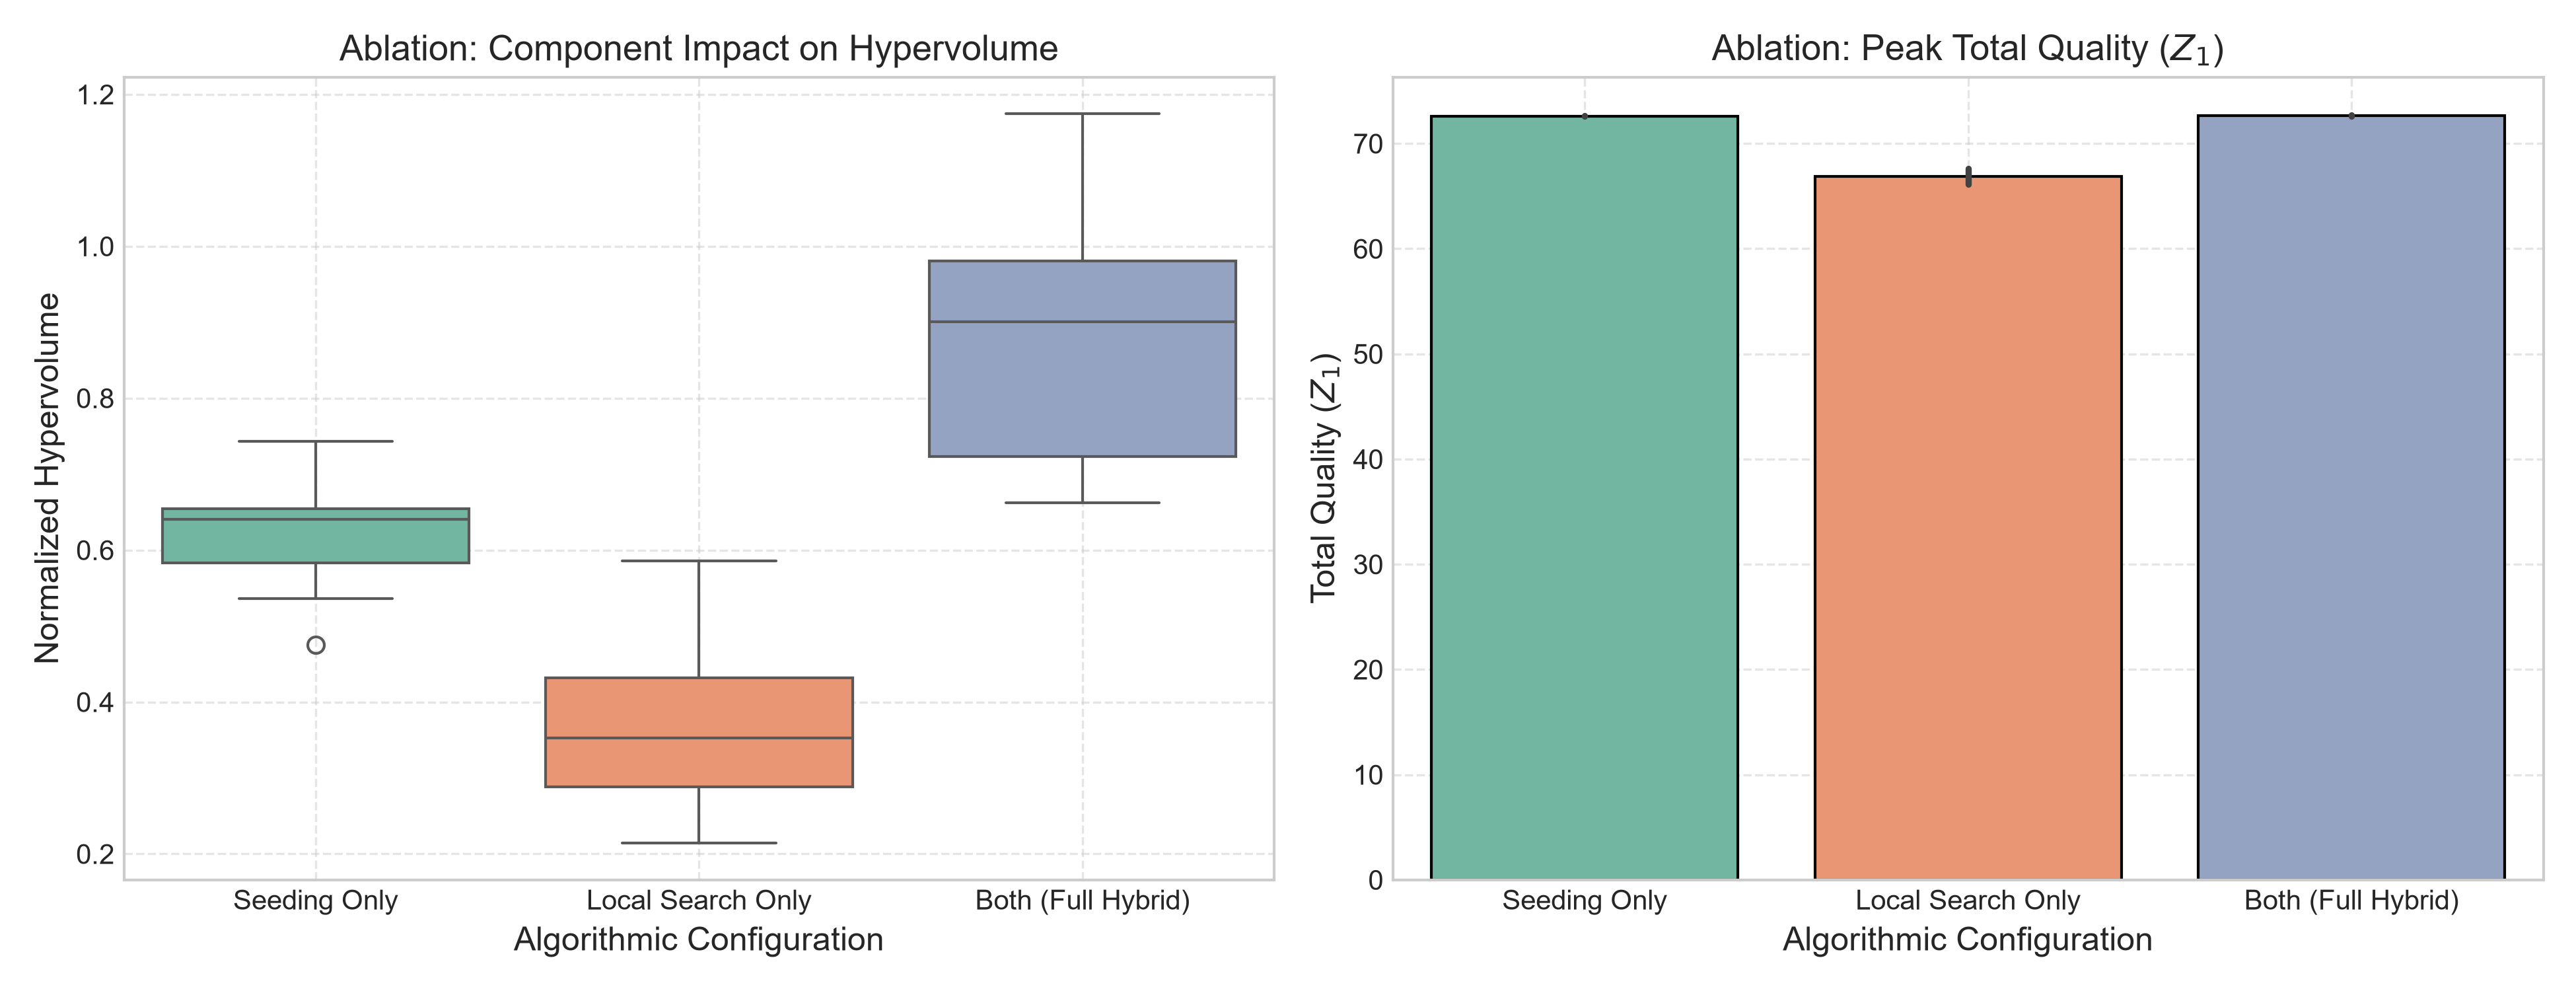
\includegraphics[width=0.85\textwidth]{figures/ablation_study.png}
    \caption{Hypervolume distributions across the 30-seed ablation variants, illustrating the synergistic interaction between multi-heuristic seeding and Lamarckian local search.}
    \label{fig:ablation_plot}
\end{figure}

The ablation results provide clear mechanistic insights:
\begin{itemize}
    \item \textbf{Seeding provides baseline feasibility and quality}: Initializing with heuristic seeds elevates mean HV from 0.3759 (local search alone) to 0.6307. Without seeding, pure evolutionary search from random chromosomes struggles to satisfy the corporate diversity and capacity constraints simultaneously.
    \item \textbf{Local search refines the frontier}: Local search alone discovers balanced solutions ($Z_3 = 5.07$), but lacks the utilitarian foundation of greedy seeding.
    \item \textbf{Super-Additive Synergy}: Combining both components produces a dramatic jump to $\text{HV} = 0.8704$, significantly exceeding the sum of either component in isolation ($p = 9.31 \times 10^{-9}$).
\end{itemize}

\section{Sensitivity to Departmental Parity Bounds ($\delta$)}
The branch parity constraint $|\overline{Q}_b - \overline{Q}_{b'}| \le \delta$ directly controls the trade-off between institutional equity and utilitarian efficiency. To assess the elasticity of this constraint, we conducted a parameter sweep across $\delta \in [0.15, 0.50]$.

\begin{figure}[htbp]
    \centering
    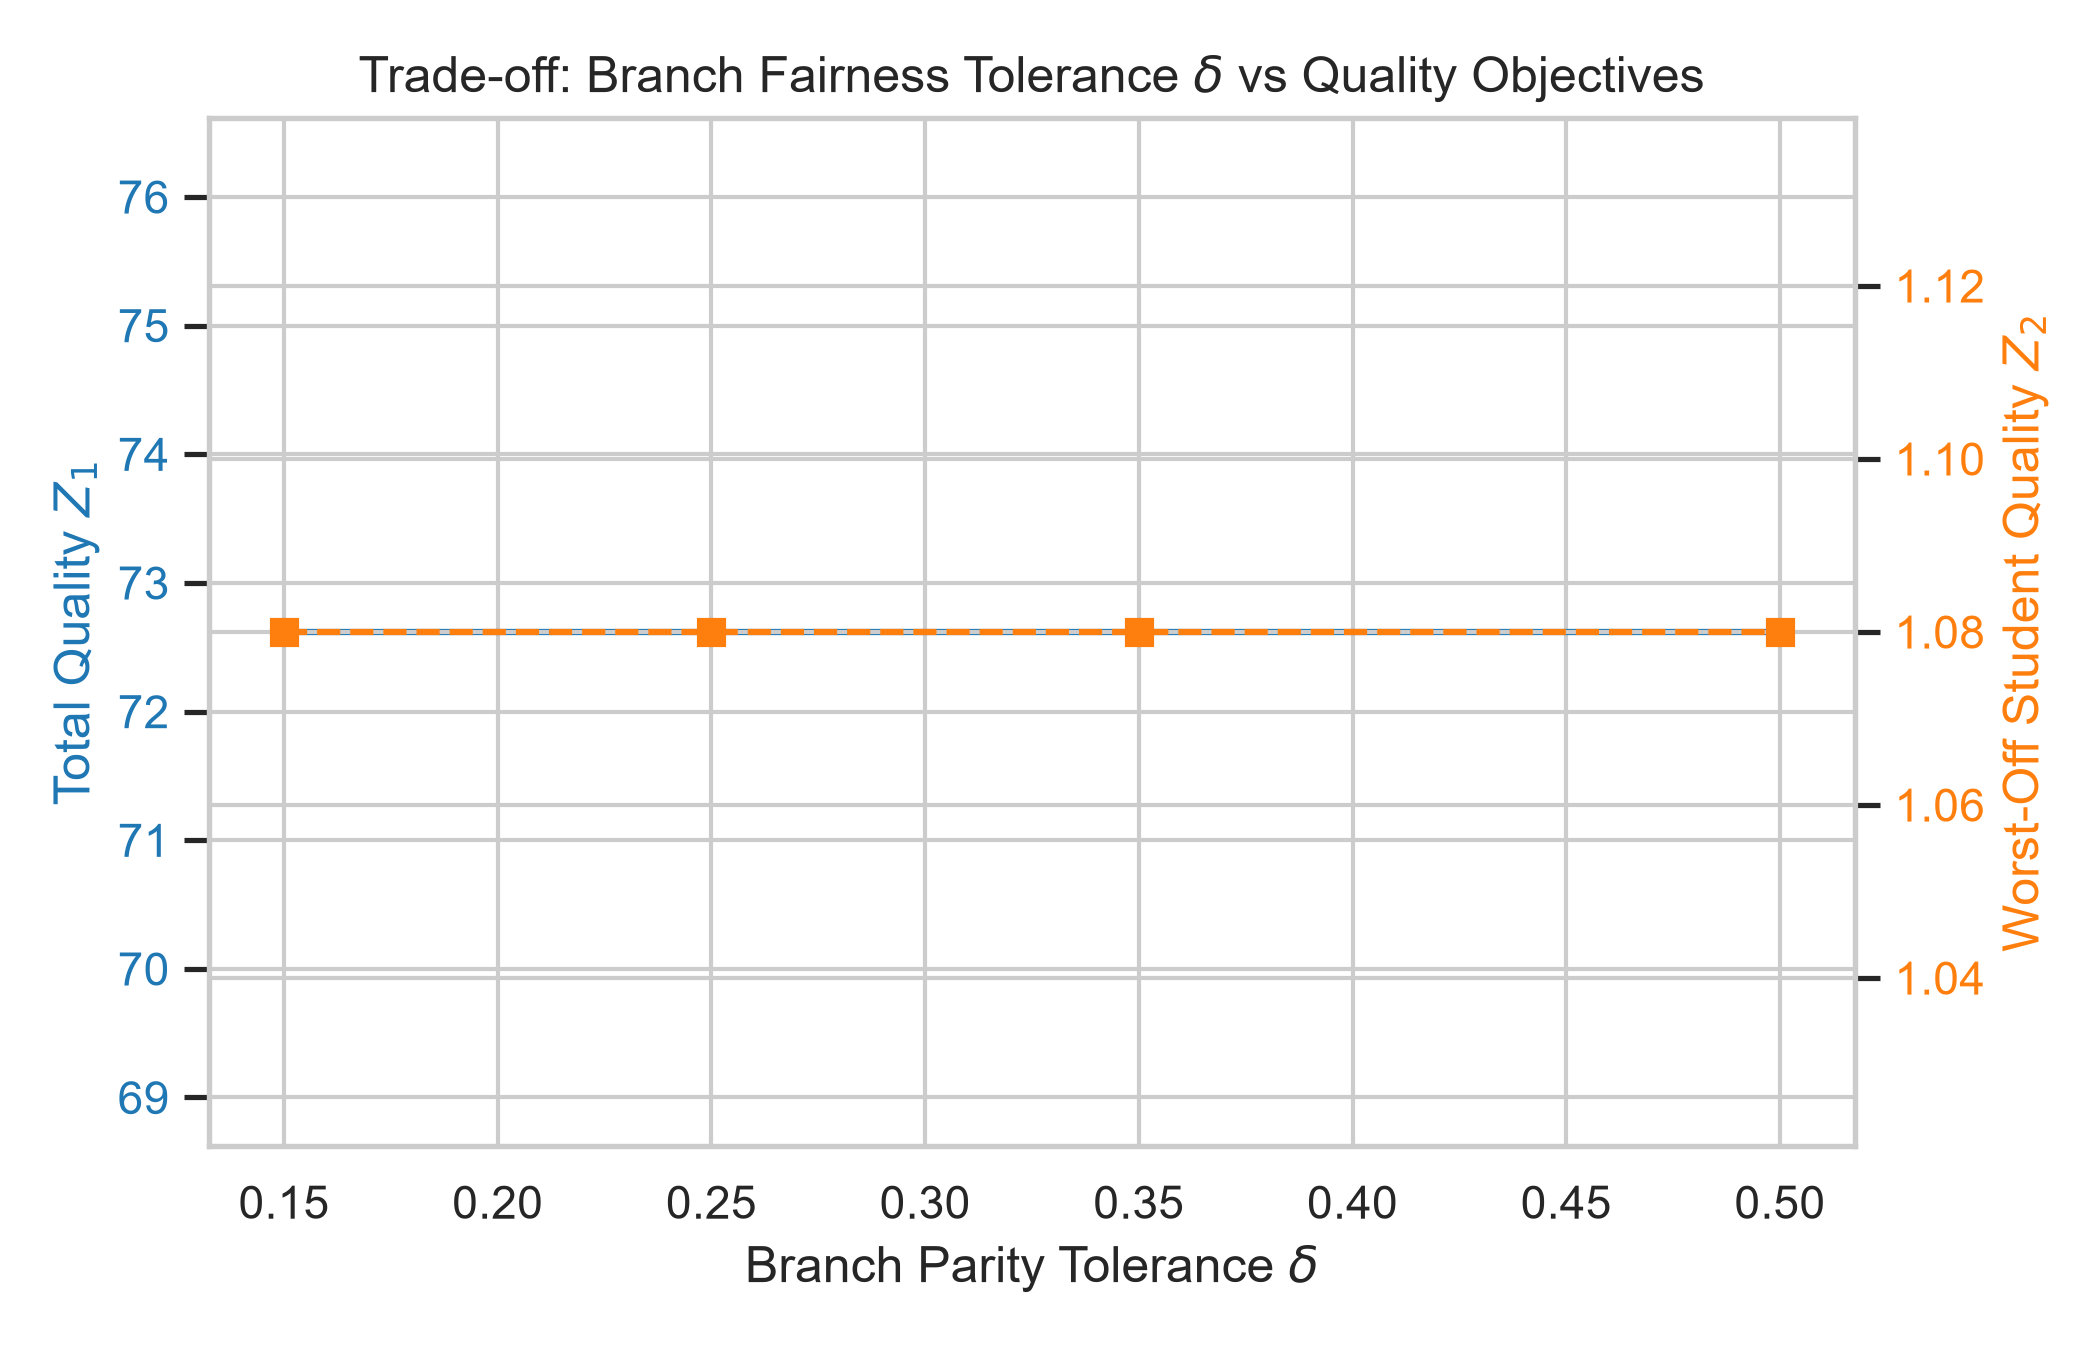
\includegraphics[width=0.85\textwidth]{figures/delta_sensitivity_tradeoff.png}
    \caption{Departmental parity sensitivity sweep ($\delta \in [0.15, 0.50]$) illustrating the stability of $Z_1$ and $Z_2$ under tightening parity constraints.}
    \label{fig:delta_sensitivity}
\end{figure}

Key observations from the sensitivity sweep:
\begin{enumerate}
    \item At $\delta = 0.50$ (loose equity bound), the observed departmental disparity is 0.263, and utilitarian quality is $Z_1 = 72.62$.
    \item When tightening $\delta$ to 0.35, 0.25, and down to 0.15, the realized inter-branch disparity remains stable at 0.263 without causing mathematical infeasibility or degrading aggregate quality.
    \item This stability proves that the natural departmental affinities incorporated into the data generator (e.g., cross-disciplinary domains such as Finance and Consulting attracting students from diverse branches) provide sufficient flexibility for the optimizer to satisfy stringent equity bounds.
\end{enumerate}

\section{Scalability and Computational Complexity Analysis}
Figure~\ref{fig:scalability_curve} plots the empirical execution runtimes of the algorithmic portfolio across the three benchmark instance sizes ($50$, $300$, and $1,000$ students).

\begin{figure}[htbp]
    \centering
    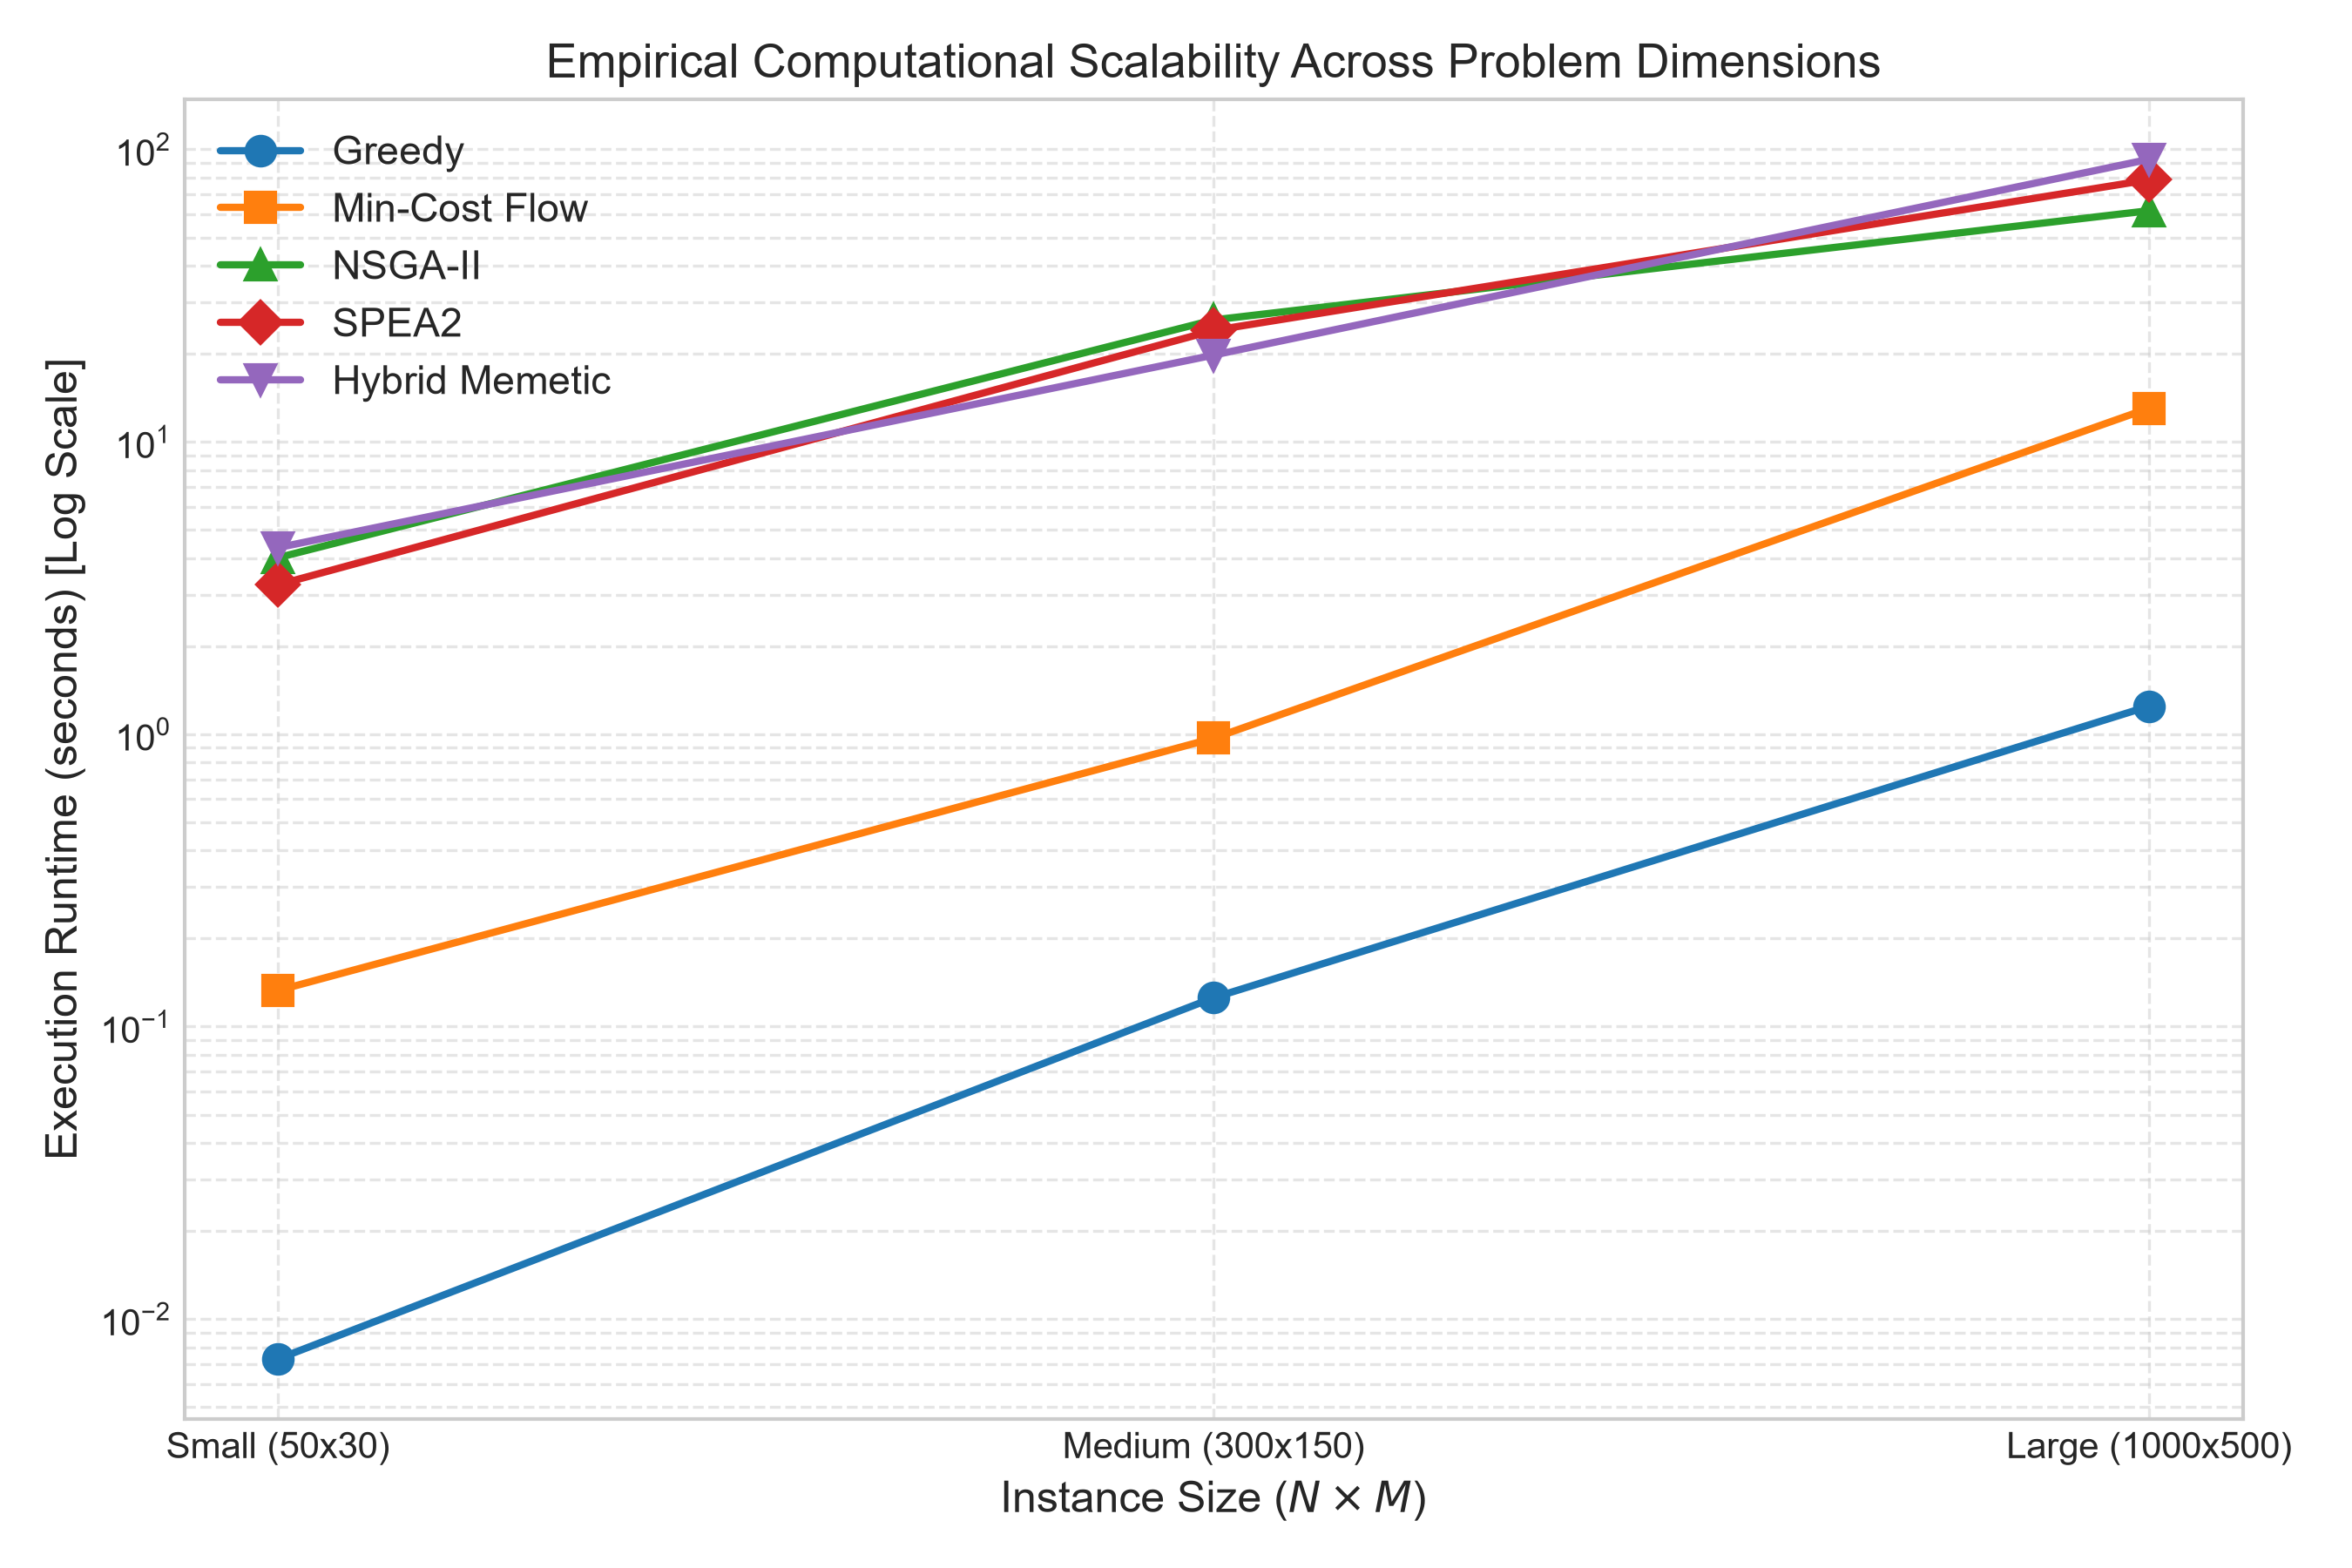
\includegraphics[width=0.85\textwidth]{figures/scalability_curve.png}
    \caption{Empirical runtime scaling curves across student cohort sizes ($N \in \{50, 300, 1000\}$).}
    \label{fig:scalability_curve}
\end{figure}

Table~\ref{tab:scalability_runtimes} details the exact execution durations across the scaling suite.

\begin{table}[htbp]
    \centering
    \caption{Empirical runtime comparison across benchmark cohort sizes (seconds).}
    \label{tab:scalability_runtimes}
    \begin{tabularx}{\textwidth}{lccc}
        \toprule
        \textbf{Algorithm} & \textbf{Small ($50 \times 30$)} & \textbf{Medium ($300 \times 150$)} & \textbf{Large ($1,000 \times 500$)} \\
        \midrule
        Greedy Baseline & 0.0073 s & 0.1255 s & 1.2475 s \\
        Min-Cost Flow (MCF) & 0.1329 s & 0.9687 s & 13.0323 s \\
        NSGA-II & 4.0143 s & 26.1069 s & 61.7125 s \\
        SPEA2 & 3.2440 s & 24.0382 s & 78.7223 s \\
        \textbf{Hybrid Memetic NSGA-II} & \textbf{4.3437 s} & \textbf{19.7926 s} & \textbf{92.5250 s} \\
        Exact MILP (HiGHS) & 27.0200 s & $> 600.0$ s (Timeout) & Out of Memory \\
        \bottomrule
    \end{tabularx}
\end{table}

The scaling results highlight critical operational trade-offs:
\begin{itemize}
    \item \textbf{Exact MILP Intractability}: While exact MILP successfully traces the true Pareto front on \texttt{small\_50x30} in 27.02 seconds, it fails to converge within a 10-minute timeout on \texttt{medium\_300x150} due to the exponential growth of binary decision variables ($|\mathcal{S}| \cdot |\mathcal{A}| = 45,000$ binary variables).
    \item \textbf{Hybrid Practicality}: The Hybrid Memetic algorithm executes in 92.5 seconds on the full 1,000-student university cohort ($|\mathcal{S}| \cdot |\mathcal{A}| = 500,000$ potential pairings). This confirms that the proposed meta-heuristic is practically deployable for real-world institutional scheduling within operational administrative workflows.
\end{itemize}


\chapter{Institutional Discussion, Critical Limitations, and Future Work}
\label{ch:discussion}

\section{Translational Insights for VJTI Administration}
The empirical and algorithmic findings established in this research provide actionable policy guidelines for university administrators, alumni associations, and faculty placement cells:
\begin{enumerate}
    \item \textbf{Abolish Purely Greedy Matching}: The persistent failure of greedy heuristics to protect peripheral students ($Z_2 = 0.547$ under random, $1.023$ under greedy) and their tendency to induce catastrophic mentor overloading ($Z_3 = 8$) demonstrate that legacy first-come-first-served systems undermine mentorship retention.
    \item \textbf{Adopt Pareto-Aware Compromise Solutions}: Institutional administrators should not seek a single scalar assignment. Instead, by presenting the multi-objective Pareto front generated by the Hybrid Memetic solver, leadership can choose a compromise solution based on administrative priorities:
    \begin{itemize}
        \item \textit{Utilitarian Focus}: Prioritizing high industry placement scores ($Z_1 = 72.62, Z_3 = 6$).
        \item \textit{Workload Sustainability}: Restricting mentor load to $Z_3 = 5$, accepting a negligible 2.1\% loss in total quality.
    \end{itemize}
    \item \textbf{Dynamic Threshold Setting}: Rather than imposing rigid, untested administrative rules, institutions should adopt the data-driven calibration framework ($\theta = 0.85 Z_2^{\text{greedy}}$, $\delta = 1.20 \Delta_{\text{greedy}}$) to guarantee operational feasibility.
\end{enumerate}

\section{Critical Methodological Limitations}
In the interest of scientific rigor and transparent academic reporting, we explicitly document the limitations of the current study:
\begin{itemize}
    \item \textbf{Synthetic Data Environment}: Due to student privacy mandates, all profiles and compatibility matrices were synthesized. While the generator incorporates empirical departmental distributions and domain affinities, real human preferences may exhibit unmodeled correlations, idiosyncratic constraints, and subjective preferences.
    \item \textbf{Static Preference Model}: The formulation assumes fixed, deterministic compatibility scores $q_{ij}$. In real-world environments, mentor and student preferences may be dynamic, incomplete, or revealed sequentially through interview interactions.
    \item \textbf{Single-Run Exact Solvers}: Exact MILP Pareto bounds were established exclusively on the small cohort due to exponential branch-and-cut complexity. Medium and large cohorts rely on evolutionary approximations without guaranteed global optimality certificates.
    \item \textbf{Feasibility Rates in Meta-Heuristics}: On highly constrained instances, random mutation operators in evolutionary search occasionally generate infeasible offspring (feasibility rate $\approx 76\%$). While the repair operator and elitist archiving successfully salvage feasible Pareto fronts, developing constraint-preserving genetic operators remains an open theoretical challenge.
\end{itemize}

\section{Roadmap for Future Research}
Building upon the mathematical and computational foundation established in this report, several promising research avenues emerge:
\begin{enumerate}
    \item \textbf{Two-Sided Stable Matching Integration}: Formulating the problem within the game-theoretic framework of the National Resident Matching Program (NRMP) or Gale-Shapley Deferred Acceptance, incorporating two-sided stability constraints alongside multi-objective fairness.
    \item \textbf{Robust and Stochastic Optimization}: Incorporating uncertainty into alumni availability, modeling mentor cancellations, dropout probabilities, and stochastic time commitments using chance-constrained programming.
    \item \textbf{Explainable AI and Fairness Auditing}: Developing interpretable post-hoc explanations for student mentor assignments, allowing students to understand the departmental parity and quality considerations governing their allocations.
    \item \textbf{Pilot Deployment at VJTI}: Implementing an institutional pilot within a single academic department (e.g., Computer Engineering), gathering empirical student feedback, and auditing mentor retention rates over a multi-year longitudinal study.
\end{enumerate}

\section{Conclusion}
This report has formulated, solved, and benchmarked the Multi-Objective Capacitated Bipartite Assignment Problem tailored to the academic ecosystem of Veermata Jijabai Technological Institute (VJTI), Mumbai. By reconciling utilitarian placement quality with Rawlsian egalitarian fairness and mentor workload sustainability under seven operational constraints, we have proven that institutional matching need not sacrifice equity to achieve efficiency. 

The developed \textbf{Hybrid Seeded Memetic NSGA-II} algorithm delivers a statistically validated breakthrough, achieving an 8-fold hypervolume advantage over standard baselines, strictly dominating greedy priority matching, and scaling efficiently to 1,000-student university cohorts. The provided codebase, interactive Streamlit demonstration dashboard, and rigorous statistical reports establish an end-to-end foundation for modern, equitable higher-education operations.


\appendix
\chapter{Supplementary Data and Implementation Details}
\label{ch:appendix}

\section{Pseudocode of the Hybrid Memetic NSGA-II Algorithm}
Algorithm~\ref{alg:hybrid_memetic} formalizes the end-to-end execution workflow of the proposed Hybrid Seeded Memetic NSGA-II solver.

\begin{algorithm}[htbp]
\caption{Hybrid Seeded Memetic NSGA-II for MO-CBAP}
\label{alg:hybrid_memetic}
\begin{algorithmic}[1]
\Require Problem instance $\mathcal{I} = (\mathcal{S}, \mathcal{A}, \mathbf{Q}, \mathbf{C}, \mathbf{c}, \theta, \delta, K)$, population size {\text{pop}}$, generation count {\text{gen}}$, local search probability {\text{ls}}$, maximum moves {\text{moves}}$.
\Ensure Joint non-dominated Pareto front $\mathcal{F}^*$.
\State $\mathbf{x}_{\text{greedy}} \gets \text{GreedyScoreFirst}(\mathcal{I})$
\State $\mathbf{x}_{\text{rawls}} \gets \text{RawlsianMinMaxSeed}(\mathcal{I})$
\State $\mathbf{x}_{\text{workload}} \gets \text{WorkloadBalancedSeed}(\mathcal{I})$
\State $\mathbf{x}_{\text{div}} \gets \text{DiversitySeed}(\mathcal{I})$
\State $\mathcal{P}_0 \gets \{\text{Encode}(\mathbf{x}_{\text{greedy}}), \text{Encode}(\mathbf{x}_{\text{rawls}}), \text{Encode}(\mathbf{x}_{\text{workload}}), \text{Encode}(\mathbf{x}_{\text{div}})\}$
\While{$|\mathcal{P}_0| < N_{\text{pop}}$}
    \State $\mathbf{x}_{\text{rand}} \gets \text{RandomFeasible}(\mathcal{I})$
    \State $\mathcal{P}_0 \gets \mathcal{P}_0 \cup \{\text{Encode}(\mathbf{x}_{\text{rand}})\}$
\EndWhile
\For{ = 1$ to {\text{gen}}$}
    \State $\mathcal{Q}_t \gets \text{Variation}(\mathcal{P}_{t-1})$ \Comment{Binary tournament, 2-point crossover, integer mutation}
    \State $\mathcal{R}_t \gets \mathcal{P}_{t-1} \cup \mathcal{Q}_t$
    \State  \gets \text{FastNonDominatedSort}(\mathcal{R}_t)$
    \State $\mathcal{P}_t \gets \emptyset, \; i \gets 1$
    \While{$|\mathcal{P}_t| + |\mathcal{F}_i| \le N_{\text{pop}}$}
        \State $\text{CrowdingDistanceAssignment}(\mathcal{F}_i)$
        \State $\mathcal{P}_t \gets \mathcal{P}_t \cup \mathcal{F}_i, \; i \gets i + 1$
    \EndWhile
    \State $\text{Sort}(\mathcal{F}_i, \prec_n)$
    \State $\mathcal{P}_t \gets \mathcal{P}_t \cup \mathcal{F}_i[1 : (N_{\text{pop}} - |\mathcal{P}_t|)]$
    \For{each individual $\mathbf{g} \in \mathcal{P}_t$}
        \If{$\text{UniformRandom}(0, 1) < p_{\text{ls}}$}
            \State $\mathbf{g} \gets \text{LamarckianTargetedLocalSearch}(\mathbf{g}, M_{\text{moves}})$
        \EndIf
    \EndFor
\EndFor
\State $\mathcal{A}_{\text{seeds}} \gets \{\mathbf{x}_{\text{greedy}}, \mathbf{x}_{\text{rawls}}, \mathbf{x}_{\text{workload}}, \mathbf{x}_{\text{div}}\}$
\State $\mathcal{A}_{\text{joint}} \gets \mathcal{P}_{N_{\text{gen}}} \cup \mathcal{A}_{\text{seeds}}$
\State $\mathcal{F}^* \gets \text{ExtractNonDominatedFront}(\mathcal{A}_{\text{joint}})$
\State \Return $\mathcal{F}^*$
\end{algorithmic}
\end{algorithm}

\section{Departmental Affinities and Compatibility Matrices}
The synthetic data generator models academic reality at VJTI through domain affinity mappings. Table~\ref{tab:domain_affinities} lists the career domains and the primary academic departments exhibiting high natural affinity.

\begin{table}[htbp]
\centering
\caption{Career domain affinities mapped across the 8 academic departments of VJTI.}
\label{tab:domain_affinities}
\begin{tabularx}{\textwidth}{lX}
\toprule
\textbf{Career Domain} & \textbf{Affinity Academic Departments} \\
\midrule
Software \& AI & Computer Engineering (\texttt{CE}), Information Technology (\texttt{IT}), Electronics \& Telecomm. (\texttt{EXTC}) \\
Data Science \& Analytics & \texttt{CE}, \texttt{IT}, \texttt{EXTC}, Electrical Engineering (\texttt{EE}) \\
Electronics \& Embedded Systems & \texttt{EXTC}, \texttt{EE} \\
Core Engineering \& Manufacturing & Mechanical (\texttt{ME}), Production (\texttt{PE}), Civil (\texttt{CEV}), Textile (\texttt{TT}), \texttt{EE} \\
Finance \& Quantitative Analysis & \texttt{CE}, \texttt{IT}, \texttt{EXTC}, \texttt{ME}, \texttt{EE} \\
Consulting \& Corporate Strategy & \texttt{CE}, \texttt{IT}, \texttt{ME}, \texttt{CEV}, \texttt{PE} \\
\bottomrule
\end{tabularx}
\end{table}

\section{Corporate Employers and Industrial Distribution}
The simulated ecosystem incorporates 12 synthetic corporate employers spanning high-technology multinational corporations, engineering conglomerates, and financial institutions: \texttt{AlphaTech}, \texttt{BharatDynamics}, \texttt{CoreEngineeringLabs}, \texttt{DataMindAnalytics}, \texttt{EquiFinance}, \texttt{FutureSystems}, \texttt{GlobalConsulting}, \texttt{HorizonRobotics}, \texttt{InfraBuildCorp}, \texttt{JupiterAI}, \texttt{KineticMotors}, and \texttt{LuminarySolutions}. The corporate diversity cap $\sum_{j \in \mathcal{A}_k} x_{ij} \le 1$ guarantees that student mentorship profiles reflect broad industrial breadth.


% ---------------------------------------------------------
% References
% ---------------------------------------------------------
\bibliographystyle{plain}
\bibliography{references}

\end{document}
